\cleardoublepage %poner esta linea al inicio de cada capitulo

\chapter{Introducción}

La agricultura ha sido uno de los pilares más importantes tanto para el desarrollo de la sociedad como para su manutención, ya que es gracias a está, que los países pueden generar empleos y aumentar sus recursos económicos, sin embargo las tareas de agricultura pueden llegar a ser tediosas o muy pesadas para las personas, es por esto que con el avance tecnológico se ha buscado mejorar el sector de la agricultura no solo para facilitar a los agricultores las tareas que deben hacer, sino también permitir que el producto ofrecido sea de mayor calidad, para garantizar que su comercialización tenga un mayor auge globalmente.\\

Uno de los principales avances tecnológicos en el sector agro-industrial, es la implementación de visión artificial en los procesos productivos, con esta se busca corregir las fallas humanas y garantizar que el producto mantenga siempre una buena y mejor calidad, que se busca garantizar con la normativa INCONTEC, la cual debe tener en cuenta para la exportación de productos agrícolas. El proyecto busca desarrollar un sistema mecatrónico implementando técnicas de visión artificial para mejorar el proceso de producción de la papa, esto podría ayudar al crecimiento del sector papicultor del país, debido a que se espera mejorar la calidad del producto y sea más eficiente su clasificación.


\newpage
\section{Objetivos}

\subsection{Objetivo General}

Implementar un prototipo para la clasificación de características de calidad en los tubérculos de papa producidos en la región Andina de Colombia, mediante técnicas de visión por computadora.

\subsection{Objetivos Específicos}
\begin{enumerate}
	\item Identificar a través de técnicas de visión artificial los rasgos de calidad "y características físicas" que se encuentran en los tubérculos de papa. 
	\item Evaluar el desempeño del prototipo propuesto para realizar la clasificación de los tubérculos de papa bajo las categorías de tamaño grande mediana y pequeña establecidas por la norma NTC341. 
	\item Comparar la precisión del modelo propuesto con modelos similares de clasificación
\end{enumerate}

\section{Alcances y Limitaciones}

\subsection{Alcances}

Para la realización del proyecto se debe tener en cuenta que se enfocará en los tubérculos de papa R12 y pastusa producidos en la región andina de Colombia. Se espera que el producto se encuentre limpio de suciedades como tierra y raíces, para llevar acabo el análisis por técnicas de visión artificial. El análisis se enfocará en identificar las características de calidad del producto para ser comercializado. Se propone un sistema mecatrónico tipo banda transportadora, para generar el desplazamiento de los tubérculos de papa por debajo de una cámara, que realiza el análisis de visión artificial y extrae las características de calidad de la papa.  

\subsection{Limitaciones}


El proyecto se encuentra limitado a los recursos de software y hardware, (computacionales), con los que cuentan los integrantes del proyecto y las plataformas open sources a las que se le puedan sacar provecho, para la implementación de los algoritmos que actualmente se encuentran en la literatura.

\section{Justificación}

En la actualidad, uno de los retos que enfrenta el sector de la agricultura es el aumento en la calidad del producto necesaria para pasar a una etapa de comercialización. Debido a que la producción de papa en Colombia aporta el $3.3 \%$ del Producto Interno Bruto (PIB), las siembras son de alrededor de $130 \ mil$ hectáreas y se cosechan cerca de $2,8$ millones de toneladas. Además, en Colombia la producción de papa genera anualmente alrededor de $264 \ mil$ empleos, aproximadamente $75 \ mil$ son trabajos directos y alrededor de $189 \ mil$ son indirectos \cite{referencia2}. El cultivo de la papa constituye el eje fundamental de la economía del país, en $283$ municipios a nivel nacional, donde se involucran más de $90 \ mil$ familias principalmente en los departamentos de Boyacá, Cundinamarca, Antioquia y Nariño, los cuales concentran más del $85 \%$ de la producción \cite{referencia1}.\\
 
La automatización de procesos en la agricultura ayudan en el rendimiento de producción, sin embargo, en la etapa de comercialización tambíen se puede implementar técnicas que mejoren faciliten la mejora de la calidad del producto. Implementando técnicas de visión artificial, se desarrollará un sistema mecatrónico que permita la selección de tubérculos de papa de forma automatizada y con mayor precisión, con el fin de mejorar el proceso actual que se lleva a cabo para la clasificación de calidad en los tubérculos de papa.


\section{Descripción y formulación del problema}
La agricultura de Colombia es un componente fundamental en la economía del territorio, ya que juega un papel primordial en el desarrollo económico del país. Debido a que es la principal fuente de ingresos del área rural, hace un aporte relevante al desarrollo económico, la mitigación de la pobreza, y el desarrollo sustentable de Colombia.\\


Uno de los sectores más grandes en la agricultura colombiana es el sector papicultor, en Colombia se caracteriza por tener poco desarrollo tecnológico y buscar abastecer el consumo interno, sin mayor exploración en mercados internacionales. Frente a la coyuntura en la que se encuentra el sector, gracias a los retos que traen consigo los acuerdos comerciales firmados por el gobierno nacional, el sector papicultor requiere urgentes transformaciones que permitan aumentar su competitividad y por ende lograr el crecimiento del sector.\\


Como consecuencia, en los últimos años, el sector agricultor de Colombia ha implementado herramientas tecnológicas que le permitan a los agricultores, aumentar la calidad de sus productos y así poder competir tanto en el mercado local como en el global. Pensando en esto, las diferentes técnicas de visión artificial, han tenido un auge en la agricultura de precisión, ayudando a clasificar productos basándose en sus diferentes características sin importar su clase, sin embargo, las técnicas de visión artificial no han sido aprovechadas para mejorar el sector papicultor colombiano.\\

El sector agricultor de Colombia ha implementado diferentes técnicas de visión artificial, las cuales ayudan a clasificar los productos mediante las características que estos poseen, sin embargo, no se han implementado estas técnicas en la fase de almacenamiento de los tubérculos de papa, la cual es importante ya que en esta fase es donde se separan los tubérculos que cumplen las condiciones de calidad de los tubérculos que se encuentran defectuosos, ya que para la comercialización de este producto deben estar clasificados bajo la norma NTC 341.\\

¿Cómo construir un prototipo para la clasificación de tubérculos de papa mediante técnicas de visión artificial?\\

¿Qué tipo de proceso de clasificación permitirá agrupar los tubérculos de papa según sus características físicas y "patologías" mediante técnicas de visión artificial?	


\chapter{Marco Conceptual}
En este capitulo se abordan algunos términos básicos necesarios, que ayuden al entendimiento y desarrollo del proyecto. 

\section{Agricultura De Precisión} El término sobre el que se inspira la agricultura de precisión, es utilizar la porción adecuada de insumos, en el instante correcto y en el sitio preciso. La agricultura de precisión, (AP), implica la utilización de sistemas de posicionamiento universal, (GPS), y de otros medios electrónicos, para obtener datos del cultivo. Las tecnologías de la agricultura de precisión, permiten saciar una de las exigencias de la agricultura actualizada. Se muestra como primordial virtud, que la exploración de resultados de los ensayos se puede hacer por sectores diferentes en un mismo lote, y tal cual ajustar el desempeño diferencial en los mismos. La utilización de las tecnologías de la agricultura de precisión puede contribuir a mejorar los márgenes de precisión, por medio de un incremento del costo del rendimiento, (cantidad o calidad), de una reducción en la proporción de insumos, o de los dos paralelamente \cite{ref_10}.

\section{Artificial Neural Networks} Las RNA son sistemas de procesamiento de la información, cuya composición y manejo permanecen inspirados en las redes neuronales biológicas. Consisten en un enorme conjunto de recursos básicos de procesamiento, denominados nodos o neuronas, que permanecen organizados en capas. De esta forma, las RNA son sistemas adaptativos que aprenden de la vivencia, en otros términos, aprenden a realizar ciertas labores por medio de un entrenamiento con ejemplos ilustrativos \cite{ref_11}.
\\ 

\section{Convolución Dilatada}

Se trata de un método que busca ampliar la entrada insertando huecos entre sus elementos consecutivos. Siendo igual que una convolución normal, pero con la diferencia de que omite pixeles, con el fin de cubrir más área de la entrada, dando un campo de visión más amplio con el mismo coste computacional, por medio de un parámetro llamado factor de dilatación \textit{l}, indicando cuanto se expande la entrada \cite{wu2019fastfcn}. La Figura \ref{fig:cd} muestra un ejemplo de la implementación de la convolución dilatada.

\begin{figure}[ht]
	\centering
	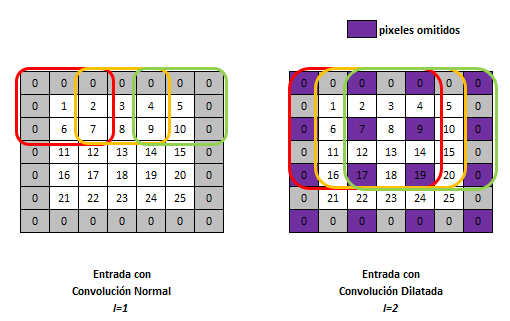
\includegraphics[scale=0.6]{Figs/Convolucion_dilatada.png}
	\caption{Ejemplo Convolución Dilatada}
	\label{fig:cd}
\end{figure}


\section{Data Augmentation}
El Data augmentation consiste en la transformación de los datos existentes, para crear un \textit{dataset} con mayor cantidad de datos diferentes. El objetivo de esta herramienta es crear nuevos datos que puedan ser añadidos al conjunto ya existente, y así contar con más muestras para un mejor desempeño del algoritmo. Además de esto, también es implementado para reducir el \textit{overfitting}, ya que al añadir más información al conjunto de entrenamiento se evita que el modelo se sobre ajuste. \\


El concepto Data Augmentation tiene relación con los procedimientos para edificar algoritmos iterativos de mejora o muestreo, por medio de la introducción de datos no vigilados o cambiantes latentes. Para los algoritmos estocásticos, el procedimiento se popularizó en la literatura estadística por el algoritmo de incremento de datos de Tanner y Wong, y en la literatura de física por el algoritmo de Swendsen y Wang, para el muestreo de los modelos de Ising y Potts y sus generalizaciones; en la literatura de física, el Data Augmentation, se conoce como el procedimiento de las cambiantes auxiliares. Generalmente, la obra de esquemas de el Data augmentation es que den sitio a algoritmos básicos y rápidos, debido a que las tácticas famosas varían de una manera significativa con respecto a los modelos.\cite{van2001art}

\section{\textit{Dropout}}

Para cada entrenamiento de redes neuronales, la propagación hacia adelante involucra la eliminación aleatoria de la mitad de activaciones en cada capa. Haciendo que el error se extienda hacia atrás a traves de las activaciones remanentes, reduciendo sustancialmente al sobreajuste. Se cree que es debido al impedimento de que los pesos de la red colaboren entre sí para memorizar las muestras del entrenamiento mejorando su rendimiento \cite{hinton2012improving}

\section{Filtro de mediana}

Es una tecnología que procesa señales no lineales. El valor del ruido que proviene de la imagen digital o la secuencia es sustituida por el valor mediano de la vecindad (máscara).\\
Los pixeles de la máscara se clasifican en el orden de sus niveles de gris, el valor mediano del grupo es almacenado para sustituir el valor del ruido \cite{zhu2012improved}.

\section{Imagen Binaria} Se define una imagen binaria como una función de dos variables discretas
a[m,n], las cuales puede tomar dos valores, ‘0’ o ‘1’, dependiendo del nivel de gris de la
imagen (una imagen binaria tiene dos niveles: blanco y negro). Existe una definición alternativa, la cual considera que una imagen consiste en un conjunto de
coordenadas discretas (también pueden ser reales pero no es el objetivo de este estudio). En este sentido, el conjunto corresponde a todos aquellos puntos o píxeles que pertenecen a la imagen. Por lo tanto, se puede decir que en morfología matemática los conjuntos representan objetos en una imagen \cite{ref_12}.

\section{\textit{Max-pooling}}

Una capa de agrupación normal, realiza un muestreo decreciente dividiendo la entrada en agrupaciones rectangulares y calculando los valores máximos de cada agrupación.\\

Un operador max-pooling, se puede usar para la reducción del muestreo sobre las bandas de salida convolucionales, haciendo una reducción de la variabilidad. Esto lo realiza a través de un valor máximo como se muestra en la Ecuación ~\ref{eq:maxp}, dentro de un grupo de activaciones A. La banda máxima agrupada m está compuesta por f filtros relacionados $p_{m}=[p_{1m},...,p_{fm}] \in A^f$.

\begin{equation}
	\label{eq:maxp}
	p_{f,m}=max(h_{f,(m-1)N+r})
\end{equation}

Donde $N \in (1,...,R) $ representado como un desplazamiento de agrupación cuando $N < R$. La capa de agrupación disminuye la dimensionalidad de salida de K bandas convolucionales a $M=(K-R)/N+1$ bandas, que han sido agrupadas teniendo como resultante $p=[p1,...,pM] \in R^{M.J}$ \cite{gholamalinezhad2020pooling}, un ejemplo de max-pooling se puede observar en la Figura \ref{mp}.

\begin{figure}[ht]
	\centering
	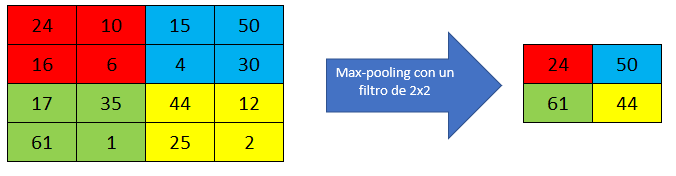
\includegraphics[scale=0.6]{Figs/mp.png}
	\caption{Ejemplo Max-Pooling}
	\label{mp}
\end{figure}

\section{\textit{Over-fitting}}

Un problema al momento de entrenar redes neuronales, es el \textit{over-fitting}, el cual se da cuando la red neuronal en un momento especifico del ciclo de entrenamiento no muestra un progreso en la capacidad de resolver problemas. Sino que solamente aprende una regularidad aleatoria dentro del conjunto de patrones de entrenamiento \cite{jabbar2015methods}.

\section{\textit{Padding}}

Se utiliza para acomodar el dominio finito de las muestras, lo cual permite que el soporte de la convolución se extienda más allá de los limites de las mismas, reduciendo el impacto de los efectos de frontera.\\

El más utilizado es el \textit{zero padding}, debido a que mantiene la misma dimensionalidad al aplicar convoluciones. Por otro lado permite a las redes neuronales convolucionadas codificar información de posición absoluta, a pesar de capas de agrupamiento en su arquitectura \cite{islam2021position}, un ejemplo de padding se puede observar en la Figura \ref{padding}.

\begin{figure}[ht]
	\centering
	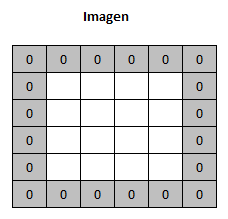
\includegraphics[scale=0.65]{Figs/padding.png}
	\caption{Ejemplo Zero-Padding}
	\label{padding}
\end{figure}


\newpage
\section{Procesamiento de imágenes} El procesamiento digital de imágenes, es el conjunto de prácticas que modifican imágenes digitales para mejorar la visibilidad de ciertas características de los objetos presentes en la imagen, para su posterior análisis o simplemente para mejorar la visualización de la
imagen.\\

El objetivo del procesamiento de imágenes no es aumentar la información que se puede extraer de las imágenes, solo se busca realzar ciertas características de la imagen. Para procesar la imagen efectivamente se debe considerar el proceso de formación y las características de interés de la imagen \cite{ref_13}.


\section{\textit{Stride}}


Es un parámetro que especifica cuántos píxeles se traslada horizontalmente y verticalmente, mientras es convolucionada la imagen. En algunas arquitecturas el \textit{stride} se utiliza en vez de \textit{max pooling} para reducir el tamaño de la capa \cite{murphy2016overview}, un ejemplo de stride se puede observar en la Figura \ref{stride}.

\begin{figure}[ht]
	\centering
	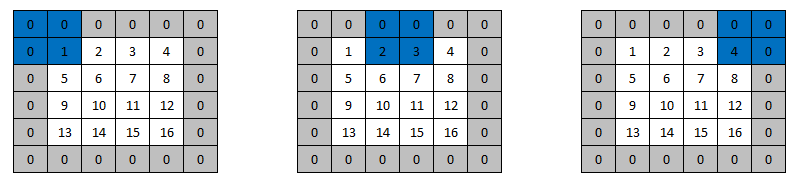
\includegraphics[scale=0.5]{Figs/stride.png}
	\caption{Convolución con Zero Padding y Stride $> 1$}
	\label{stride}
\end{figure}

\newpage
\section{Transfer Learning}
El aprendizaje por transferencia, se define como la mejora del aprendizaje en una nueva tarea, a través de la transferencia de conocimientos de una tarea relacionada que ya se ha aprendido. Aunque la mayoría de los algoritmos de aprendizaje automático están diseñados para abordar tareas individuales, el desarrollo de algoritmos que faciliten el aprendizaje por transferencia, es un tema de interés permanente en la comunidad de aprendizaje automático. El aprendizaje por transferencia se utiliza para mejorar a un alumno de un dominio, mediante la transferencia de información de un dominio relacionado. Se puede tener en cuenta experiencias no técnicas del mundo real para entender por qué es posible el aprendizaje por transferencia.\\

Como en el caso del aprendizaje semisupervisado, los métodos de aprendizaje por transferencia se utilizan cuando hay una escasez directa de los datos de entrenamiento subyacentes. Sin embargo, la diferencia con el aprendizaje semisupervisado, es que en lugar de utilizar datos sin etiquetar, se utilizan datos etiquetados de un dominio diferente para mejorar \cite{ref_14}.

\section{\textit{Thresholding}}


Es un método que divide una imagen en grupos parecidos según un conjunto de criterios ya definidos. Podemos encontrar varias técnicas de \textit{Thresholding} teniendo un enfoque primordial de la segmentación, especialmente en aplicaciones en las que la velocidad es fundamental en el proceso. \textit{Thresholding} puede ser adaptativo al utilizarse diferentes umbrales para distintas regiones de la imagen \cite{kulkarni2012color}.


\section{\textit{Under-fitting}}

Es lo contrario al \textit{over-fitting}, siendo este cuando el modelo creado es incapaz de percibir variabilidad alguna en los datos. Dando como resultado que el clasificador resultante no tenga la capacidad de realizar una predicción aceptable \cite{jabbar2015methods}.

\section{Visión artificial} La visión artificial o visión por computador, intenta replicar la capacidad que tienen algunos seres vivos para visualizar una imagen, entenderla y actuar con base en lo observado. Existe un crecimiento en los diferentes tipos de aplicaciones industriales que requieren el uso de técnicas de visión artificial. El  continuo  desarrollo  de  nuevos  algoritmos  y  aplicaciones,  hacen  de  esta  disciplina  una tecnología en constante evolución, la cual ha experimentado un rápido avance en las últimas décadas, así lo demuestran las numerosas investigaciones y publicaciones existentes en la comunidad científica.  Esto podría deberse a la gran cantidad de contenido visual como imágenes y video que se genera en  la  actualidad,  así  como  la  capacidad  de  procesamiento  y  almacenamiento  que  tienen  los dispositivos electrónicos y la disponibilidad de herramientas, librerías y lenguajes de programación para dicho fin \cite{ref_15}.






\chapter{Estado del arte}

El objetivo de los antecedentes, es analizar y realizar una revisión literaria sobre lo  que  se  ha hecho  a  nivel  teórico  y  práctico  en  cuanto a  la visión artificial en agricultura de precisión.  Además,  determinar  cuáles son los aportes que éstos le puedan dar a este trabajo de investigación.


\section{MatLab.}

Comenzando por la literatura con temática en el procesamiento de imágenes, se tiene el trabajo de \textit{J. porras, A. Morian} \cite{article3}, en donde se menciona que la implementación de MATLAB\textsuperscript{\textregistered} como una herramienta de procesamiento de imágenes, radica en su facilidad para realizar cambios a las imágenes, es por esto qué diseñó un sistema para la clasificación de objetos con base en su forma y color, usando métodos de visión artificial en MATLAB\textsuperscript{\textregistered}, con el uso de la librería \textit{ufm.dll}, para capturar y procesar imágenes. El artículo de \textit{C. Nandi} \cite{inproceedings} presenta una investigación en dónde se consiguió calcular el tamaño de diferentes mangos, estimando el área cubierta en una imagen binaria, (imagen digital que tiene únicamente dos valores posibles para cada píxel), con base en el número de píxeles, luego de ser procesadas las imágenes, se clasificaron implementando un algoritmo basado en \textit{fuzzy logic}, teniendo en cuenta 5 variedades diferentes de mangos y como referencias el color de la cascara, tamaño, defectos superficiales, forma, firmeza, peso y olor.\\

\section{Artificial Neural Networks.}
En cuanto a la clasificación, se deben usar técnicas de visión artificial y en primer lugar, se revisó literatura  acerca de ANN, (\textit{Artificial Neural Networks}), como el trabajo de \textit{L. Pencue-Fierro y J. León Téllez} \cite{article2}, en donde se aborda una investigación hecha en Perú, en donde se aplicó visión artificial usando ANN como método de clasificación de las principales características extraídas de las frutas, que son derivadas del análisis de las superficies, tanto en su contenido cromático como en la cantidad y distribución de defectos externos. En el trabajo publicado en la revista textit{Multimedia Tools and Applications} \cite{Shrivastava2017}, donde presentaron un sistema de visión artificial que usa un enfoque de categorización simplificado con un elevado índice de exactitud. El propósito del sistema es clasificar los granos de trigo de las especies \textit{triticum aestivum} y \textit{triticum durum} según sus propiedades visuales, usando una ANN del tipo MLP, (\textit{Multilayer Perceptron}); las imágenes se obtienen por medio de una cámara que captura las propiedades de tamaño, color y textura de cada grano con el objeto de que sirvan de acceso al procedimiento de categorización. Otro trabajo es el publicado por \textit{Ksh. Robert Singh y Saurabh Chaudhury} \cite{Singh2016}, en donde se propone el uso de redes neuronales BPNN, (\textit{Back Propagation Artificial Neural Networks}), como método de clasificación y la descomposición mediante ondículas, (Tipo especial de transformada matemática que representa una señal en términos de versiones trasladadas y dilatadas de una onda finita), para clasificar los granos de arroz. El modelo de clasificación implemento una red neuronal BPNN de cuatro capas la cual presento mejores resultados en comparación con otros métodos.\\

Por último, usando el método de clasificación ANN, se tiene el trabajo hecho por \textit{Krzysztof Koszela} \cite{Przybyl2019}, donde se presenta una forma para garantizar la correcta clasificación de los productos y reducir las pérdidas durante su almacenamiento. La investigación abarca esfuerzos centrados en la evaluación sensorial de patatas, con el análisis de imágenes por ordenador y la modelización neuronal ANN. El objetivo de este estudio fue desarrollar un método para asistir a la identificación de cualquiera de las variedades y la turgencia de los tubérculos de patata, (Fenómeno que ocurre cuando una célula se dilata debido a la presión ejercida por los fluidos y por el contenido celular sobre las paredes de la célula), llevado a cabo sobre la base de los datos gráficos codificados en forma de imágenes digitales, obtenidos mediante algoritmos que interpretan los descriptores de imagen.\\

\section{Super Vector Machine.}
Otro método de clasificación revisado en la literatura es el de SVM \textit{Super Vector Machine}), como el usado en el trabajo de \textit{Tao Liu} y otros investigadores \cite{LIU201679}, en donde realizaron un proceso para analizar granos de arroz. El procedimiento usa 4 fuentes de luz para crear la sombra del grano en 4 direcciones; la diferencia en medio de las siluetas de los granos llenos y no llenos, se evalúa por medio del estudio de imágenes y un clasificador SVM. El análisis se hace mediante el uso de imágenes RGB, (Red-Green-Blue), de los granos con las siluetas, luego se segmentan desde la imagen binaria, para sustraer información como el sector del grano y de la sombra. En el documento publicado por \textit{Chia-Lin}  y otros investigadoores \cite{CHUNG2016404}, se menciona un método para clasificar plántulas, (Embrión ya desarrollado como consecuencia de la germinación de una semilla), sanas e infectadas. Consiste en el análisis de imágenes mediante un escáner y el proceso de clasificación utilizando SVM, en donde se hace uso de dos clasificadores, el primero distingue entre las plantas sanas y contaminadas, por otra parte, el segundo mide los niveles de contaminación. En el trabajo de \textit{Rillian Diello y Lucas Pires} \cite{PIRES201648}, se propuso un método de detección automática de enfermedad en cultivos de soja, el cual se basa en descripciones locales, conocido como el método BOV, (Bag of Values), luego de escanear la hoja. Se obtuvo a través de los vectores de entrada una clasificación en dos categorías, enfermo y sano, a partir de un clasificador SVM. Y por último, en este tipo de clasificador, el trabajo de \textit{Chengming Sun y Tao Liu} \cite{SUN2014426}, se propone un sistema para analizar el porcentaje de granos en el arroz que se encuentran en condiciones para ser distribuidos. El algoritmo se encarga de la división de los granos de manera automática. Tras la segmentación, es viable obtener el número de granos presentes en la imagen y la información específica, la exactitud del procedimiento puede verse afectada si el germen no se extrae del todo, por esa razón, el sistema detecta la viable región de germen y estima esta información usando SVM.\\

\section{Otros métodos}
En la literatura se encontraron artículos que usaban más de un método de clasificación, un ejemplo es el trabajo hecho por \textit{Tao Liu y Wen Chen} \cite{LIU201682}, el cual puso en práctica un método para controlar la población de pulgones, (Familia de insectos hemípteros), en el trigo, usando los métodos SVM, el algoritmo MSER, (\textit{Maximally Stable Extremal Regions}), y el HOG, (\textit{Histogram of Gradients}). El uso de estos 3 métodos se conoce como SMH, (Unión entre SVM, MSER y HOG), se basa en el análisis de imágenes, tratadas a partir de unos parámetros, con la finalidad de detectar la presencia y/o ausencia de pulgones, se hizo uso de este método a partir del color y la densidad de población. Al comparar este método con otros cinco comúnmente utilizados, los resultados presentaron un rendimiento superior en la identificación de pulgones. \\

De igual manera, el artículo de \textit{Rodica Sobolu} \cite{sobolu2020automatic}, propone un algoritmo de clasificación automática de patatas. Se realizaron dos tipos de clasificación: una en función del tamaño de las patatas y otra en función de su calidad. La segmentación de las zonas defectuosas se hizo mediante métodos como \textit{global thresholding}, para extraer características morfológicas y estadísticas de las zonas segmentadas. Estas características se eligieron como entradas para los algoritmos de clasificación, en donde se usaron los métodos SVM, \textit{Decision  Tree} y LDA, (\textit{Linear Discriminant Analysis}), implementados en MATLAB\textsuperscript{\textregistered} Classification Toolbox. Se llegó a la conclusión de que la SVM ha clasificado las patatas según su tamaño con una mayor tasa de éxito. En el caso de la clasificación por calidad, se recomienda el método LDA.\\

Los anteriores son los métodos más comunes que se encontraron en la literatura investigada, sin embargo, hay unos métodos poco comunes como por ejemplo los presentados en el artículo de \textit{Alberto Martines Rodriguez} \cite{article5} en donde se identificaron objetos en movimiento mediante la ayuda de la visión artificial y la transmisión de datos a un brazo robótico implementando \textit{C++} y \textit{Open CV}, usando el código de cadena, (Actualmente el grupo de reconocimiento de patrones e inteligencia artificial aplicada), para calcular las características de los objetos por color y forma. También, el artículo hecho por \textit{L. Han y M. S. Haleem} \cite{7237209}, que se usa para la detección automática, fue necesario hacer uso inicialmente de separar el fondo de la hoja, para este proceso se usó el algoritmo MCW, (\textit{Marker-Controlled Watershed}). El SLIC, (\textit{Simple Linear Iterative Clustering}), se utilizó para obtener las características presentadas por la enfermedad sobre la planta y por ultimo, la clasificación y textura se obtienen a través de GLCM, (\textit{Gray Level Co-occurrence Matrix}), el modelo de clasificación fue el SVM, este método propuesto presento un mayor rendimiento.\\

El último artículo revisado es presentado por \textit{Michael Barnes y Tom Duckett} el \cite{Barnes2010}, cuyo objetivo de  investigación es introducir un método automático de detección de manchas en imágenes digitales de patatas. El sistema desarrollado es entrenable, de modo que pueda trabajar con diferentes variedades de patatas y variaciones en las estaciones, condiciones de iluminación, etc. Otro objetivo, pensando en su posible implantación en entornos industriales, es permitir el procesamiento de imágenes en tiempo real, posiblemente mediante la construcción de \textit{Minimalist Boosted Classifier}, que extraigan un subconjunto mínimo de todas las características que optimicen el rendimiento de la detección con el menor coste computacional posible.

\section{Recolección de papa en la actualidad}

La papa es un tubérculo conocido mundialmente, con una enorme producción y valores nutritivos, contiene muchos micro nutrientes primarios y cruciales como vitamina, vitamina B6, niacina, ácido fólico, potasio, hierro y magnesio, que es una fuente importante de carbohidratos, vitaminas y minerales para el ser humano.\\
\\
En el transcurso del crecimiento, la cosecha, el transporte y el tratamiento postcosecha del tubérculo, se generan daños como cáscara verde, germinación, pudrición seca, etc.…, defectos que terminan en una reducción drástica en la calidad de venta. Tener un control de este producto es fundamental para aumentar el valor de este y generar un crecimiento en su comercialización.\\
\\
El control de calidad actualmente se realiza de forma manual, realizado por personas, clasificando según su defecto y tamaño, esta acción tiene algunas desventajas: es subjetiva, laboriosa y lleva bastante tiempo, llevando a que la clasificación decaiga con el tiempo \cite{refjaither}.



\chapter{Diseño Del Algoritmo de Clasificación}


Se diseñó un algoritmo de clasificación utilizando Redes Neuronales Convolucionales y técnicas de visión artificial con la librería \textit{Open CV}, para clasificar las características de tipo, daño y tamaño de tubérculos de papa. El Procedimiento que se llevó acabo se presenta en la Figura \ref{fig:flujogeneral}, cada ítem será explicado en las siguientes secciones. 


\begin{figure}[ht]
	\centering
	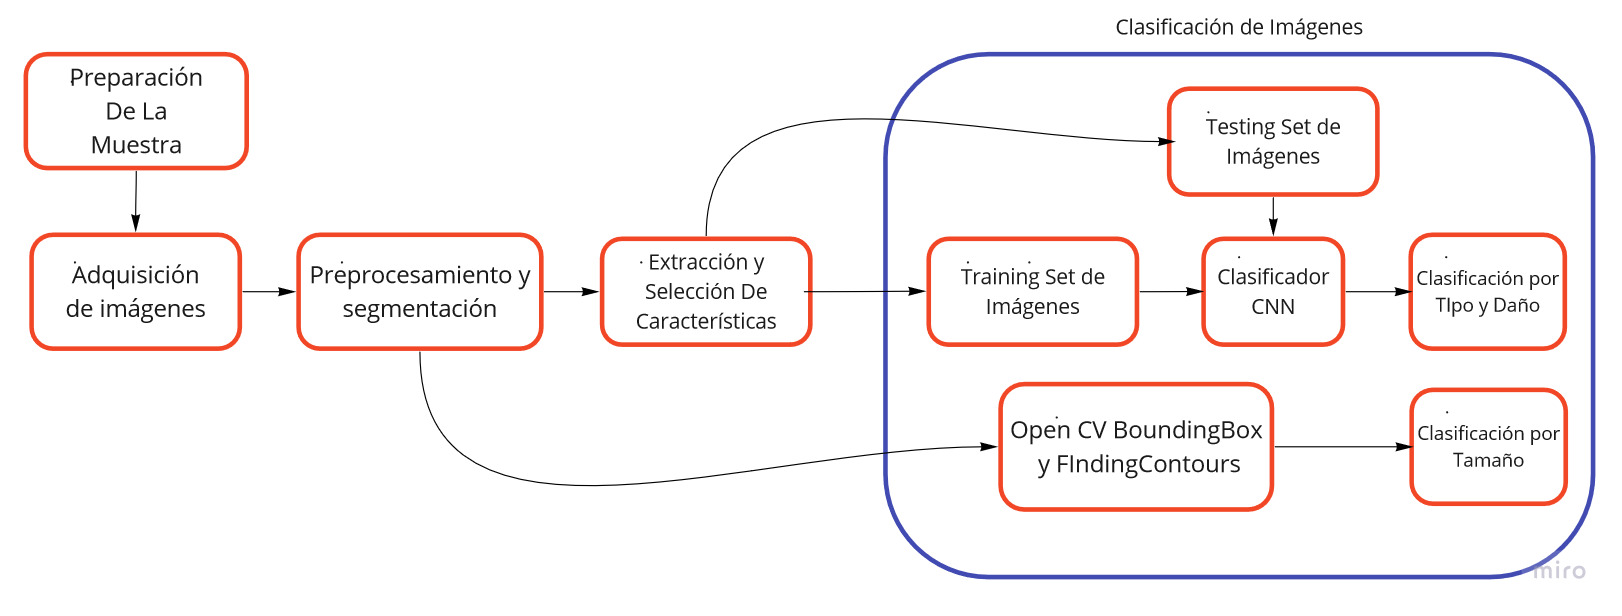
\includegraphics[scale=0.3]{Figs/FGGeneral.jpg}
	\caption{Arquitectura del Sistema de Clasificación}
	\label{fig:flujogeneral}
\end{figure}

El sistema propuesto para realizar la clasificación de tubérculos de papa en este documento, consiste desde la adquisición de muestras y creación de un dataset de tubérculos de papa, hasta el diseño de un algoritmo de clasificación con Redes Neuronales, utilizando la librería \textit{Pytorch} y la librería \textit{Open CV} de \textit{Python}. Será implementado en un prototipo de banda transportadora, que permita el movimiento de los tubérculos de papa para ser clasificados, mediante un microcontrolador y una cámara. Los sistemas de Visión Artificial que se destinan a realizar inspecciones visuales, permiten que el proceso sea más eficiente si requieren alta velocidad, gran aumento en cantidad de producción y en funcionamiento las 24 horas del día o la repetibilidad de las medidas \cite{artificial2012aplicacion}.


\section{Preparación y Adquisición De Las Imágenes}

Se preparó un total de 592 tubérculos de papa, que manualmente fueron clasificados en tres categorías definidas. Las etiquetas de cada imagen se encuentran dentro del nombre de cada archivo, que corresponde al metadata de cada foto tomada. Definido de la siguiente manera:

\begin{itemize}
	\item \textit{Tipo:} Pastusa o R12 $[0,1]$
	\item \textit{Daño:} Buena y Defectuosa $[0,1]$
	\item \textit{Tamaño:} Muy grande, Grande y Mediana $[0,1,2]$
	\item \textit{Numero de la Imágen} Etiqueta asignada por la cámara.
\end{itemize}	

Las fotos tomadas para la creación del \textit{Dataset}, poseen un tamaño de (3168, 4752) pixeles. Fueron tomadas con una cámara profesional \textit{Canon EOS 50D}, que tiene 15.1 mega pixeles de resolución y se puede ajustar la sensibilidad ISO desde 100 hasta 3200. La cámara fue configurada con ISO-800 que corresponde al parámetro de sensibilidad del sensor de ruido de la cámara, una velocidad de obturación de $\frac{1}{640}$ segundos, que corresponde al dispositivo que controla el tiempo en el que la luz incide sobre el sensor de la cámara, y finalmente una apertura de diafragma de $F-7.1$ que corresponde a la apertura del lente que deja pasar la luz \cite{Camara}, tener en cuenta que a mayor apertura de diafragma, menor luz se deja pasar. Se construyó una caja con iluminación fija la cual se muestra en la Figura \ref{fig:chamber} usando bombillos de luz blanca, de $6500$ Kelvin de temperatura de color, para que la iluminación en todas las fotos tomadas fuera uniforme, y la cámara fue fijada a un trípode ubicado a $30 \ cm$ de la base, para que la distancia del lente de la cámara con respecto a la muestra de papa fuera siempre la misma en las 592 fotos.

\begin{figure}[ht]
	\centering
	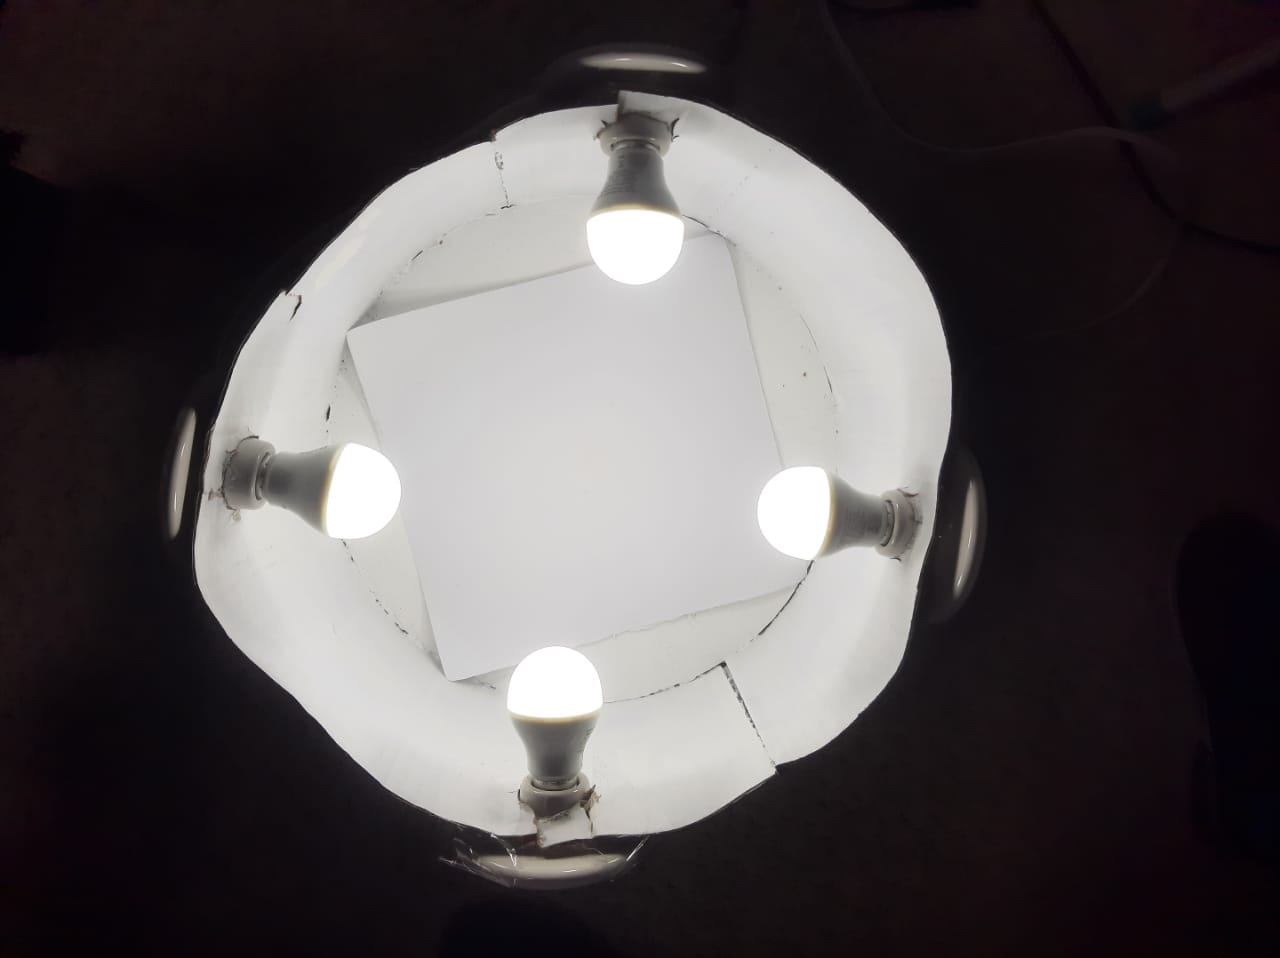
\includegraphics[scale=0.15]{Figs/Chamber.JPEG}
	\caption{Récamara Para la Toma de Fotos}
	\label{fig:chamber}
\end{figure}

Utilizando la librería \textit{Pandas} de \textit{Python}, se creó un \textit{Dataframe} que contiene el metadata de cada imagen. En la Tabla \ref{table:metadata} se puede apreciar la distribución del \textit{MetaData} de las imágenes almacenas en el \textit{Dataset}, donde se toman cinco imagenes al azar como muestra. A partir de esta tabla se crea un archivo \textit{.CSV} donde se encuentra la información de las 592 imágenes.

\begin{table}[ht]
	\centering
	\begin{tabular}{|c|c|c|c|}
		\hline
		Tipo & Daño & Tamaño & Filename \\
		\hline
		R12 & Defectuosa & Grande & 1\_1\_1\_075.JPG \\
		\hline
		PASTUSA & Buena & Grande & 0\_0\_1\_1973.JPG \\
		\hline
		R12 & Buena & Grande & 1\_0\_1\_2054.JPG \\
		\hline
		PASTUSA & Buena & Mediana & 0\_0\_2\_2042.JPG \\
		\hline
		PASTUSA & Buena & Grande & 0\_0\_1\_1955.JPG \\
		\hline
	\end{tabular}	
	\caption{MetaData de 5 Imágenes de Muestra}
	\label{table:metadata}
\end{table}


Una vez la información de cada imagen fue guardada en el archivo \textit{metadata.csv}, se agruparon las posibles combinaciones de las características de \textit{Tipo} y \textit{Daño}, para definir las \textit{clases} dentro de la red neuronal. Para realizar este proceso, se creó una condición dentro del \textit{Dataframe}, que contiene el \textit{Metadata} para generar una columna adicional con la información de la Tabla \ref{table:Clases}.	

\begin{table}[ht]
	\centering
	\begin{tabular}{|c|c|c|c|c|}
		\hline
		PASTUSA & R12 & Buena & Defectuosa & Clase \\
		\hline
		X &  & X &  & CLASE 1 \\
		\hline
		X &  &  & X & CLASE 2 \\
		\hline
		& X & X &  & CLASE 3 \\
		\hline
		& X &  & X & CLASE 4 \\
		\hline
	\end{tabular}	
	\caption{Clases Definidas}
	\label{table:Clases}
\end{table}	

De esta forma se definieron las $4 \ clases$ que serán entrenadas en la red neuronal, para el posterior proceso de clasificación por visión artificial. 


\newpage
\section{Distribución del Dataset}

Para determinar la distribución total del dataset, con el uso de la librería \textit{Plotly}, se crearon gráficas para determinar el porcentaje de imágenes pertenecientes cada característica definida en el \textit{Dataset}. La Figura \ref{fig:distribuciontipo}

\begin{figure}[ht]
	\centering
	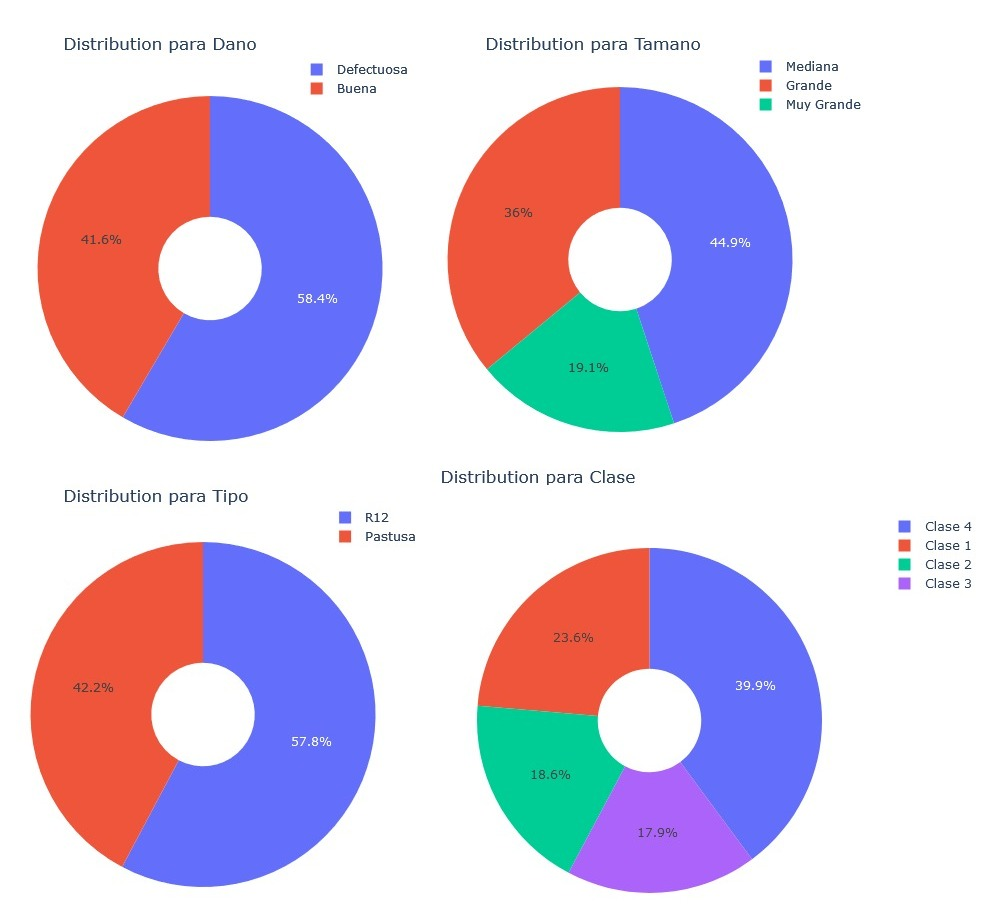
\includegraphics[scale=0.4]{Figs/Distribucion.jpg}
	\caption{Distribución del Dataset Según Sus Características Y Clases Definidas}
	\label{fig:distribuciontipo}
\end{figure}

Se definieron los \textit{Set's} de \textit{Train} y \textit{Test}, que fueron creados para el entrenamiento y validación de la red neuronal, a partir del archivo \textit{metadata.csv} de la Tabla \ref{table:metadata}. Se utilizó $80\%$ para \textit{Train} y $20\%$ para \textit{Test}. Se crearon los archivos \textit{train.csv} y \textit{test.csv} que contienen el \textit{metadata} y la dirección de las imágenes separadas en el respectivo $80\%$ y $20\%$.



\chapter{Algoritmo de Clasificación}

Se desarrolló una red neuronal artificial, (\textit{CNN}), para clasificar las características de tipo y daño, de los tubérculos de papas descritos en el \textit{Metadata}, Tabla \ref{table:metadata}. En este capitulo se presenta la definicion y estructura de una red neuronal artificial convolucional, la preparación del dataset implementado durante el entrenamiento de la red neuronal y los diferentes modelos implementados en el desarrollo del proyecto.

\section{Red Neuronal Artificial Convolucional}

La arquitectura general de una red artificial convolucional, (\textit{CNN}), se muestra en la Figura \ref{fig:cnnarchitecture} \cite{cnnarchitecture}. Se realizaron pruebas con las arquitecturas \textit{Alexnet}, \textit{Resnet18}, \textit{VGG11} y \textit{VGG19} y se implementó la optimización bayesiana en ciertos hiperparámetros de las arquitecturas existentes, para mejorar los resultados. 

\begin{figure}[ht]
	\centering
	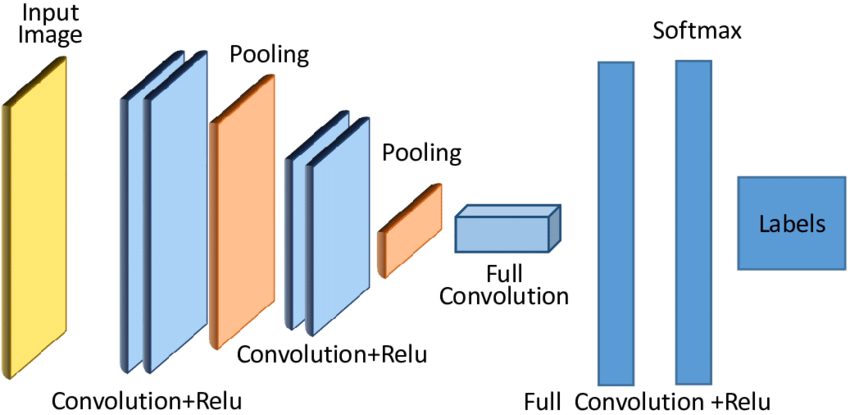
\includegraphics[scale=0.15]{Figs/A-generic-CNN-Architecture.png}
	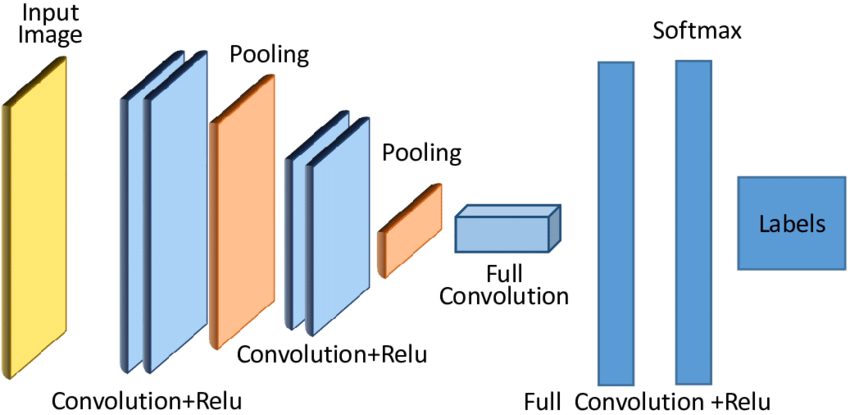
\includegraphics[scale=0.18]{Figs/A-generic-CNN-Architecture.png}
	\caption{Arquitectura General De Una CNN}
	\label{fig:cnnarchitecture}
\end{figure}	

El procedimiento realizado para desarrollar la red neuronal, se aprecia en la Figura \ref{fig:procedimiento}, donde se indican los pasos a seguir, previo a implementar alguna de las arquitecturas. Cada ítem será descrito en las próximas secciones.  

\begin{figure}[ht]
	\centering
	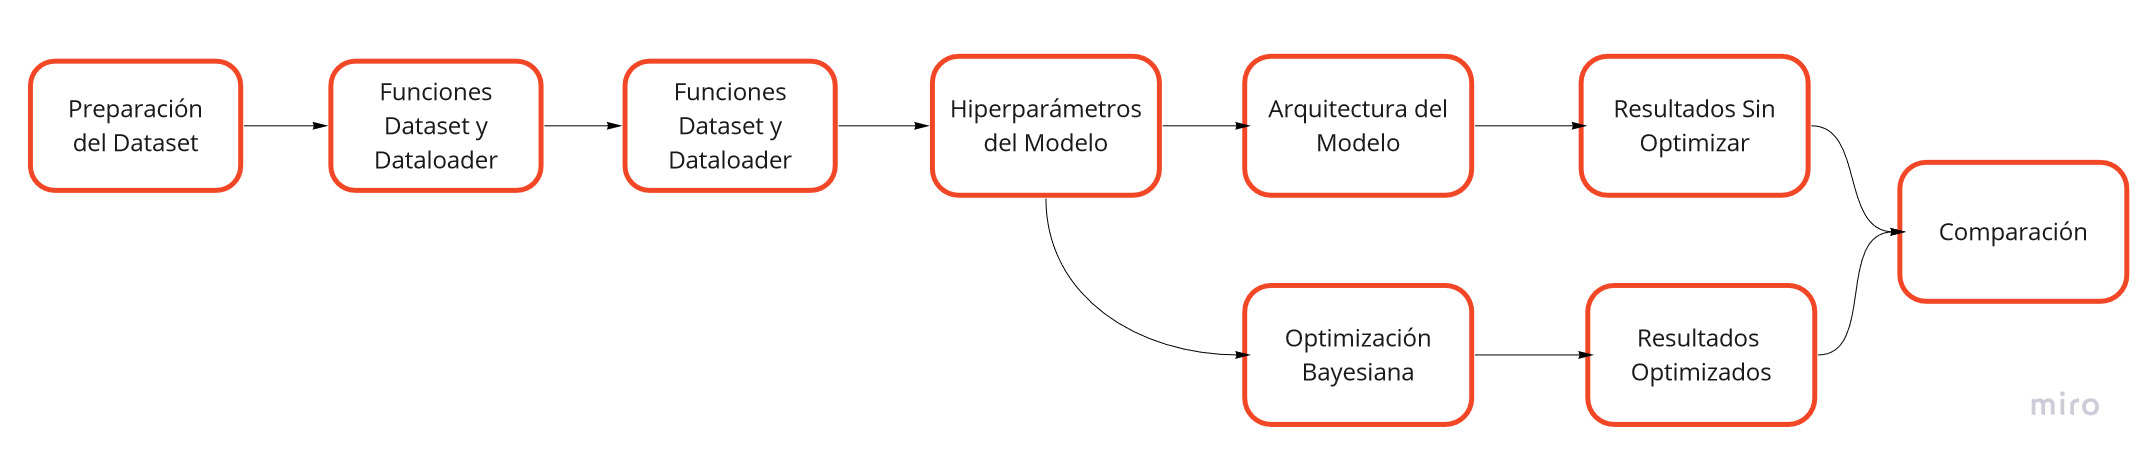
\includegraphics[scale=0.15]{Figs/procedimiento.jpg}
	\caption{Procedimiento Diseñado Para Implementar La \textit{CNN}}
	\label{fig:procedimiento}
\end{figure}	


\newpage
\subsection{Preparación Del \textit{Dataset}}

Para realizar un correcto entrenamiento de un modelo de red neuronal, es necesario aplicar un preprocesamiento a las imágenes para que el modelo extraiga características pertinentes a las clases definidas. En este apartado se explica como se lleva acabo el preprocesamiento de imágenes y los diferentes filtros aplicados para realizar el Data Augmentation.

\subsubsection{PREPROCESAMIENTO DE IMÁGENES}

Usando el módulo \textit{tranforms.compose()}, de la librería \textit{Pytorch}, se pueden encadenar unas determinadas funciones, que aplican diferentes tipos de filtros y transformaciones al \textit{Dataset}. De esta forma, se crea la tarea de segmentación debido a que las transformaciones aumentan en consideración el tamaño original del \textit{Dataset}, facilitando así, la extracción de características. Las transformaciones disponibles se presentan en la Tabla \ref{table:Filters1}.

\begin{table}[ht]
	\centering
	\begin{tabular}{|p{3cm}|p{4cm}|p{3.8cm}|p{4cm}|}
		\hline
		Image Transform       & \multicolumn{1}{c|}{Use}                                                               & Image Transform       & \multicolumn{1}{c|}{Use}                                                                        \\ \hline
		CenterCrop            & Recorta la imagen en el centro                                                         & RandomResizedCrop     & Recorta una porción aleatoria de la imágen y la redimensiona a un tamaño determinado            \\ \hline
		ColorJitter           & Cambia aleatoriamente el brillo, el contraste, la saturación y el tono de una imagen   & RandomRotation        & Rota la imagen a un ángulo determinado                                                          \\ \hline
		FiverCrop              & Recorta la imagen en cuatro esquinas y el recorte central                              & RandomVerticalFlip    & Voltea verticalmente la imagen al azar con una probabilidad dada                                \\ \hline
		Grayscale             & Convierte la imágen en escala de grises                                                & Resize                & Redimensiona la imagen al tamaño dado                                                           \\ \hline
		Pad                   & Rellena la imágen en todos sus lados con el valor de "pad" dado                        & TenCrop               & Recorta la imagen dada en cuatro esquinas y el recorte central \\ \hline
		RandomAffine          & Transformación afín aleatoria de la imagen manteniendo el centro invariante            & GaussianBlur          & Desenfoca la imágen con un filtro gausseano                                                                                                                     \\ \hline
	\end{tabular}
	\caption{Funciones de transformación de imágenes del módulo de \textit{Pytorch}}
	\label{table:Filters1}
\end{table}

En la Tabla \ref{table:Filters1} se observa una parte de las transformaciones de imágenes disponibles en el módulo \textit{torchvision.tranforms.compose} de la librería \textit{Pytorch}. En el caso del \textit{Dataset} de papas creado, se deben tener en cuenta únicamente las transformaciones cuyo resultado sea relevante para la extracción de características de la imágen, por ejemplo, como se explicó anteriormente, se va a clasificar el tubérculo de papá en tipo y daño, con la red neuronal, por este motivo, el color es una característica que define si la papa pertenece a la clase \textit{R12} o \textit{Pastusa} y, en algunos casos, si se encuentra con algún tipo de daño, por este motivo, los filtros que transforman la imágen en escala de grises no son relevantes y podrían afectar el rendimiento del algoritmo.

\begin{table}[ht]
	\centering
	\begin{tabular}{|p{3.5cm}|p{3.5cm}|p{3.8cm}|p{3.5cm}|}
		\hline
		Image Transform       & \multicolumn{1}{c|}{Use}                                                               & Image Transform       & \multicolumn{1}{c|}{Use}                                                \\ \hline
		Randomcrop            & Recorta la imágen aleatoriamente                                                       & RandomInvert          & Invierte los colores de la imágen de forma aleatoria                    \\ \hline
		RaandomGrayscale      & Convierte la imágen en escala de grises aleatoriamente                                 & RandomPosterize       & Reduce el número de bits de cada canal de laa imágen de forma aleatoria \\ \hline
		HorizontalFlip  & Voltea horizontalmente la imágen al azar con una probabilidad dada                     & RandomSolarize        & Invierte aleatoriamente el valor de los pixeles por encima de un umbral \\ \hline
		RandomPerspective     & Realiza una transformación de perspectiva aleatoria de la imagén                       & RandomAutocontrast    & Autocontraste de los píxeles de la imagen dada aleatoriamente           \\ \hline
		AdjustSharpness & Ajusta la nitidez de la imágen de forma aleatoria                                      & RandomEqualize        & Equaliza el histograma de la imágen dada aleatoriamente                 \\ \hline
		RandomApply           & Aplicar aleatoriamente una lista de transformaciones con una probabilidad determinada. & \multicolumn{1}{l|}{} &                                                                         \\ \hline
	\end{tabular}				
	\caption{Funciones de transformación de imágenes del módulo de \textit{Pytorch}}
	\label{table:filters2}
\end{table}

\newpage
De igual forma, en la Tabla \ref{table:filters2}, se observan algunos filtros como recortes en la imágen, rotaciones, cambios de perspectiva, cambios en la nitidez y contraste de la imágen. Se escogieron los filtros considerados mejores, (No cambian la morfología del color), para el caso del \textit{Dataset} de tubérculos de papa creado en este documento. Los filtros que se utilizaron en el desarrollo del algoritmo de clasificación, teniendo en cuenta aquellas transformaciones que podrían afectar el rendimiento del algoritmo son:

\begin{itemize}
	\item Resize
	\item ColorJitter
	\item RandomRotation
	\item GaussianBlur
	\item RandomPerspective
	\item RandomAdjustSharpness
\end{itemize}

Como se está utilizando la librería \textit{Pytorch}, las imágenes deben ingresar en formato \textit{Tensor}, que convierte los valores de los píxeles de una imágen \textit{PIL} estándar, con un rango de $[0, 255]$,  a un tensor decimal de \textit{Pythorch}, con valores en un rango con valores $[0.0, 1.0]$ de la forma  $(C, H, W)$, siendo C el número de canales de la imágen, (1 si es en escala de grises, 3 si es \textit{RGB}), $H$ y $W$ el tamaño de la imágen. \\

Una vez la imágen está en formato \textit{PyTorch FloatTensor}, se decidió utilizar la función \textit{torchvision.tranforms.normalize()} para normalizar las imágenes. La normalización de una imágen consiste en modificar los valores del tensor, que se encuentran entre $[0.0, 1.0]$, para que el promedio y la desviación estándar sean $0$ y $1$ respectivamente. Para hacer esto se utiliza la Ecuación \ref{eq:normalize} \cite{Pytorch}

\begin{equation}
	{output[Channel]=\frac{Input[Channel]-Mean[Channel]}{std[Channel]}}
	\label{eq:normalize}
\end{equation}

La normalización se utiliza debido a que ayuda a los datos a estar definidos dentro de un rango y reducir la asimetría entre ellos, lo que permite un aprendizaje más rápido. Se diseñó una función en \textit{Python} que calcula el promedio y la desviación estándar, para \textit{Trainset} y para el \textit{Testset}. De esta forma se garantiza que la normalización sea correcta en el total del \textit{Dataset}. Los valores obtenidos para el \textit{Trainset} Ecuación \ref{eq:meanstd1} y el \textit{Testset} Ecuación \ref{eq:meanstd2} respectivamente.

\begin{equation}				{mean = [0.7467, 0.7389, 0.7432] \hspace*{1cm}  std  = [0.1288, 0.1633, 0.2045]}
	\label{eq:meanstd1}
\end{equation}


\begin{equation}
	{mean = [0.7507, 0.7430, 0.7486] \hspace*{1cm}  std  = [0.1265, 0.1609, 0.2012]}
	\label{eq:meanstd2}
\end{equation}

La Figura \ref{fig:agumentation} enseña una matriz de imágenes como parte del \textit{Trainset}, que muestra las transformaciones hechas al $80\%$ de las imágenes del \textit{Dataset}, y la clase a la que pertenece la Tabla \ref{table:Clases}, verificando así que las funciones creadas están enlazando correctamente la imágen con su respectiva clase y aplicando de forma correcta las transformaciones.


\begin{figure}[ht]
	\centering
	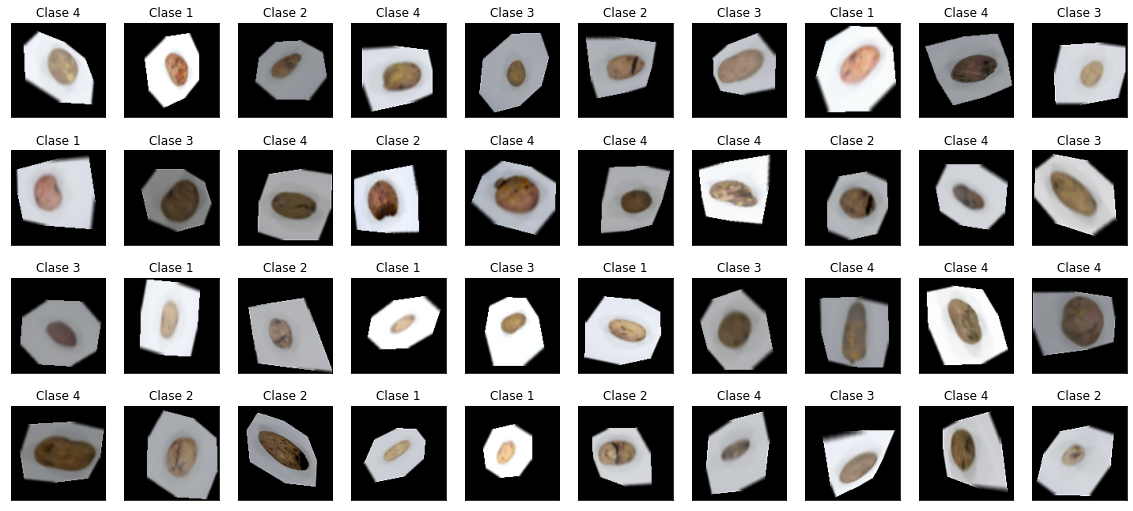
\includegraphics[scale=0.4]{Figs/augmentation.png}
	\caption{Matriz de Imágenes Con Transformaciones Aplicadas}
	\label{fig:agumentation}
\end{figure}	

\subsection{Funciones PotatoDataset y DataLoader}

Una vez se realiza el proceso de \textit{Data Augmentation}, se deben cargar las imágenes en \textit{Pytorch} para que puedan ser procesadas por el modelo de red neuronal. En este capítulo se presenta la creación de la función \textit{PotatoDataset()}, y la implementación de la función \textit{Dataloader}, ademas de la explicación de cada función, para cargar el conjunto de datos en \textit{Pytorch}.


\subsubsection{FUNCIÓN POTATODATASET}

Se creó una clase, (\textit{Python Class Object Constructor}), con el nombre de \textit{AttributesDataset()}, que se encarga de leer el \textit{Metadata}  de cada imágen y convertirlo en \textit{labelID}, en la Tabla \ref{table:metadata} se muestra como son ingresadas las imágenes en el algoritmo, sin embargo, las características deben ser ingresadas como \textit{labelID}, es decir, el label Pastusa corresponde al ID 0 en la categoría de Tipo. Este diccionario se presenta a continuación:			

\begin{itemize}
	\item Tipo: ${'Pastusa': 0, 'R12': 1}$
	\item Daño: ${'Buena': 0, 'Defectuosa': 1}$
	\item Tamaño: ${'Muy Grande': 0, 'Grande': 1, 'Mediana': 2}$
\end{itemize}

En la red neuronal, únicamente se utilizaron \textit{labels} y \textit{labelID} de tipo y daño para definir las clases de la Tabla \ref{table:Clases}. La función \textit{Dataset} de \textit{Python} realiza el proceso de cargar y relacionar cada imágen con su respectivo \textit{label}, para \textit{Dataset's} que se encuentran organizados dentro de carpetas jerarquicamente. El \textit{Dataset} creado en éste documento no se encuentra organizado de esta manera, sino que la organización jerárquica que define las clases se encuentra dentro del \textit{metadata}, en el nombre de cada imágen, Tabla \ref{table:metadata}, debido a esto es que se desarrolló una función que cargara y relacionara de la misma manera que lo hace la función integrada de \textit{Pythorch}. Esta función fue llamada \textit{PotatoDataset()}, que utiliza los \textit{labelID} generados por la función \textit{AttributesDataset()}, y carga cada imágen relacionada con sus \textit{labelID}. Como se desarrolló la función, de igual forma debe ser capaz de aplicar las transformaciones a cada imágen. El objeto regresa las 592 imágenes cargadas en \textit{Python}, cada una relacionada con su respectivo \textit{labelID} y \textit{label}, y con una transformación o múltiples aplicadas. Esta función desarrollada, cuenta con los mismos atributos iterables que poseen los \textit{dataset's} creados a partir de la función integrada en \textit{Pytorch}.			


\subsubsection{FUNCIÓN DATALOADER}			

Generalmente, una vez se finaliza el proceso de cargar las imágenes utilizando la función \textit{DataSet} de \textit{Pytorch}, se procede a utilizar la función \textit{DataLoader} para generar múltiples lotes de imágenes, a partir de las transformaciones utilizadas. La función \textit{DataLoader()}, de \textit{Pytorch}, es implementada para realizar la importación de datos a gran escala. Para el uso de esta función se debe tener en cuenta que el argumento más importante será el \textit{dataset}, que fue generado por el objeto \textit{PotatoDataset()}. \\

Según como se explico en el apartado anterior, se generó un \textit{dataset} del tipo \textit{iterable-style Datsets}, lo que permite utilizar la función integrada \textit{DataLoader()} de \textit{Pytorch}. El \textit{DataLoader} permite la agrupación automática de muestras de datos individuales obtenidas en los \textit{Batch's} mediante argumentos. Los \textit{DataLoader's} cuentan con una gran catidad de argumentos que ayudan a que la carga de datos sea más eficiente \cite{Pytorch}. Es por esta razón, que para la ejecución de este dataloader se implementaron los parámetros de la Tabla \ref{table:Argumentos}.
\newpage			
\begin{table}[ht]
	\centering
	\begin{tabular}{|p{3cm}|p{8cm}|}
		\hline
		FUNCIÓN & DESCRIPCIÓN \\ 
		\hline
		Batch size & Cuántas muestras por Batch hay que cargar (Default: 1)\\
		\hline
		Shuffle & Se establece en TRUE para que los datos se reorganicen en cada época (Default: FALSE)  \\
		\hline
		Num workers & Cuántos subprocesos se utilizarán para la carga de datos. 0 significa que los datos se cargarán en el proceso principal. (Default: 0)\\
		\hline
	\end{tabular}	
	\caption{Argumentos para el Dataloader}
	\label{table:Argumentos}
\end{table}

Los argumentos explicados en la tabla \ref{table:Argumentos} fueron establecidos de la siguiente forma:

\begin{itemize}
	\item $Batch \ Size = 40$
	\item $Shuffle = True$
	\item $Num \ workers = 0$
\end{itemize}

Esto con el objetivo de que el \textit{Dataloader} cargue 40 muestras por época, y tome otras 40 diferentes para la siguiente época, y así sucesivamente hasta terminar todas las épocas establecidas.  





\subsection{Hiperparámetros Del Modelo}

La mayor parte de modelos implementados en machine learning, poseen una serie de parámetros que no pueden ser aprendidos de los datos, es por esto que deben ser establecidos antes del entrenamiento. Estos parámetros son conocidos como hiperparámetros. En este capítulo se abordan los hiperparámetros utilizados en el desarrollo de este proyecto.

\subsubsection{FUNCIÓN DE PÉRDIDAS}		

\textit{Pytorch} posee una cantidad interesante de funciones de pérdidas, para su uso en la clasificación de clases en redes neuronales. Una función de pérdidas, evalúa la desviación entre las predicciones realizadas por la red neuronal y los valores reales de las muestras utilizadas durante el entrenamiento de la red. Cuanto menor sea el valor de la función, es más eficiente la red neuronal \cite{mathivet2018inteligencia}. 	
Para el desarrollo de la red neuronal, se utilizó la pérdida de entropía cruzada entre la entrada y el objetivo \cite{Pytorch}. Es útil cuando se entrena un problema de clasificación con más de una clase.  El objetivo que espera este criterio debe contener:

\begin{itemize}
	\item Índices de clase en el rango $[0,C)$ donde $C$ es el número de clases.
	\item Probabilidades de clase se requieren más allá de una sola clase cuando se encuentran etiquetas combinadas.				 
\end{itemize}

En cada lote usado en el entrenamiento de la red neuronal, se encuentran etiquetas combinadas en el \textit{Metadata} de las imágenes, como se describió en la Tabla \ref{table:Clases}, por lo tanto, una función de pérdida no reducida \cite{Pytorch} se describe en la Ecuación ~\ref{eq:perd}.\\

\begin{equation}
	\label{eq:perd}
	{l_n=-\sum_{c=1}^{C}w_c log\left(\frac{exp(x_n,c)}{\sum_{i=1}^{C}exp(x_n,i)}y_n,c\right)}
\end{equation}\\

Donde $x$ es la entrada, $y$ el objetivo de predicción, $w$ es el peso, $C$ el número de clases y $N$ es la dimensión del \textit{Batch}. Usando la función \textit{nn.CrossEntropyLoss()}, se calculan las pérdidas entre entrada y salida del modelo entrenado, para posteriormente utilizar estas pérdidas como métricas en porcentajes de \textit{Accuracy} y \textit{Losses}.\\			

El rendimiento de esta función de pérdidas, es mejor cuando el objetivo contiene índices de clase y no las etiquetas, ya que esto permite optimizar el cálculo, por esta razón, se agruparon las etiquetas de las imágenes en $4 \ Clases$ definidas.

\subsubsection{OPTIMIZADOR}

\textit{Pytorch} posee el paquete \textit{torch.optim}, que implementa varios algoritmos de optimización basados en el gradiente descendiente. A menudo se ha propuesto, por ejemplo Rumhart \cite{rumelhart1986learning}, minimizar el riesgo empírico $E_n(fw)$ utilizando el gradiente descendiente. Consiste en cada iteración actualizar los pesos $w$,como se muestra en la Ecuación ~\ref{eq:GD1}.


\begin{equation}
	\label{eq:GD1}
	{w_{i+1}=w_i-\gamma\frac{1}{n}\sum_{i=1}^{n}\nabla Q(z_i,w_t)}
\end{equation}\\

Donde $\gamma$ es la taza de aprendizaje elegida adecuadamente (\textit{learning rate}). Cuando la estimación inicial $w_0$ está lo suficientemente cerca del óptimo y cuando la tasa de aprendizaje es suficientemente pequeña, este algoritmo alcanza una convergencia lineal.\\


En el algoritmo desarrollado en este documento, se utilizó el optimizador de descenso estocástico del gradiente $SGD$, que es una simplificación drástica del algoritmo del gradiente descendiente. En lugar de calcular exáctamente el gradiente de $E_n(fw)$, cada iteración estima este gradiente sobre la base de un único ejemplo $z_t$ elegido al azar \cite{bottou2012stochastic}.

\begin{equation}
	\label{eq:SGD1}
	{w_{i+1}=w_i-\gamma_t\nabla_w Q(z_t,w_t)}
\end{equation}

Se espera que la Ecuación~\ref{eq:GD1} se comporte como la Ecuación~\ref{eq:SGD1} a pesar del ruido introducido por este procedimiento simplificado. El algoritmo estocástico no necesita recordar qué ejemplos de datos fueron usados durante las iteraciones anteriores, por lo tanto, puede procesar ejemplos sobre la marcha en un sistema implementado. En esta situación, el descenso estocástico del gradiente optimiza directamente el riesgo esperado.	

\subsection{Arquitectura del modelo}

Se utilzaron modelos pre definidos para realizar el entrenamiento del \textit{Dataset}, utilzando la teoría de \textit{Transfer Learning} que permite entrenar los modelos, con pesos establecidos entrenadas para otro tipo de datos, para obtener resultados a partir de ellos sin empezar desde cero la creación de una red neuronal y sus pesos. En este capítulo se presenta la estructura y los resultados obtenidos de los modelos pre entrenados AlexNet, VGG-19, VGG-11 y ResNet-18, sin el uso de un método de optimización de hiperparámetros.

\subsubsection{\MakeUppercase{Modelo preentrenado ALEXNET}}

El modelo AlexNet fue implementado en el año 2012 en el desafió de reconocimiento visual a gran escala Imaget. Este modelo tuvo un resultado tan satisfactorio, que los modelos de aprendizaje profundo, se convirtieron en la referencia para la investigación y desarrollo en los principales sectores de la industria. \cite{Pytorch}\\


El modelo se compone de cinco capas convolucionales y tres capas densas, donde las capas convolucionales están normalizadas por lotes. El kernel tiene dimensiones diferentes que se distribuyen en \textit{11 x 11} en la primera capa, \textit{5 x 5} en la segunda y \textit{3 x 3} en las demás. La primera, cuarta y quinta capa convolucional, están seguidas por una capa Max-pooling con dimensiones de \textit{3 x 3}, que posee un stride de dos.\\


Las capas convolusioonales y de Max-pooling son seguidas por tres capas densas, en donde las dos primeras poseen 4096 neuronas cada una y la ultima capa es la de salida, la cual se compone de 1000 neuronas que poseen una función de activación softmax. Estas neuronas son las encargadas de realizar la clasificación de la imagen. Como es habitual en estos sistemas de clasificación, la función de perdidas implementada es la entropía cruzada \cite{ref_1}.\\

\newpage

\begin{figure}[ht]
	\centering
	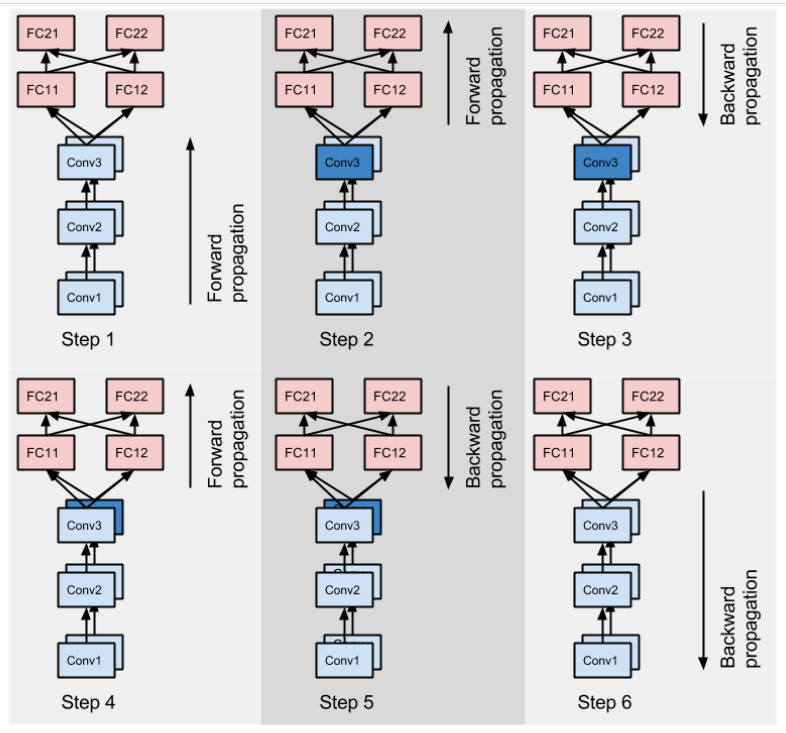
\includegraphics[scale=0.4]{Figs/5.png}
	\caption{Modelo AlexNet}
	\label{fig:AlexNet}
\end{figure}

Como se aprecia en la Figura \ref{fig:AlexNet}, el modelo de AlexNet, toma una imagen de entrada con una resolución de \textit{227 x 227} pixeles y 3 canales de color, la información recibida pasa por cinco capas convolucionales, (en negro), de neuronas ReLu y tres capas de Max-pooling, (en azul). La quinta capa de convolución posee 256 mapas diferentes con dimensiones de \textit{13 x 13}. Seguidamente se aplican las dos capas densas de 4096 neuronas, las cuales son seguidas por una capa de salida de 1000 neuronas, dotadas con una función softmax. Cada neurona de la capa de salida representa un conjunto semántico diferente. Y su valor de activación indica la probabilidad de que la imagen de entrada pertenezca a dicho conjunto semántico.\\


\subsubsection{\MakeUppercase{Modelo preentrenado VGG19}}

La arquitectura VGG fue planteada por Simonyan y Zisserman, la cual consiste en stacks lineales de bloques, que se encuentran formados por una cantidad determinada de capas convolucionales, una función de activación no lineal y una capa Max Pooling, seguidos de tres capas fully-conected y finalmente una capa softmax \cite{ref_2}. Esta arquitectura cuenta con cinco bloques los cuales están distribuidos como se muestra en la Figura \ref{fig:VGG19}.				

\newpage
\begin{figure}[ht]
	\centering
	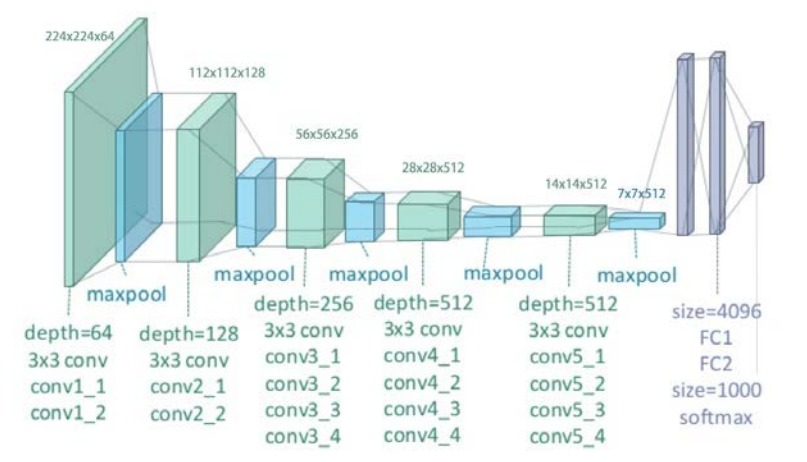
\includegraphics[scale=0.38]{Figs/22.jpeg}
	\caption{Modelo VGG19}
	\label{fig:VGG19}
\end{figure}			


Como se puede observar, la arquitectura cuenta con dos capas convolucionales de 64 y 128 filtros respectivamente, en sus dos primeros bloques, el bloque intermedio se compone de tres capas convolucionales de 256 filtros, y los últimos dos bloques están compuestos por tres capas concolucionales de 512 filtros cada uno. El numero 19 representa la cantidad de capas entrenables que posee la arquitectura, donde hay 16 capas convolucionales y 3 capas fully-conected.\\			

Las capas convolucionales de esta arquitectura presentadas en la Figura \ref{fig:VGG19}, cuentan con un campo receptivo de \textit{3 x 3}, stride de \textit{1 x 1} y pading de 1 pixel. Para la operaciones del Max Pooling se implementa un kernel de \textit{2 x 2} y un stride de \textit{2 x 2}, y por ultimo cada capa oculta de la red cuenta con la función de activación ReLu. la Figura \ref{fig:VGG19_accuracy}, muestra la precisión obtenida del entrenamiento hecho sobre esta arquitectura.


\begin{figure}[ht]
	\centering
	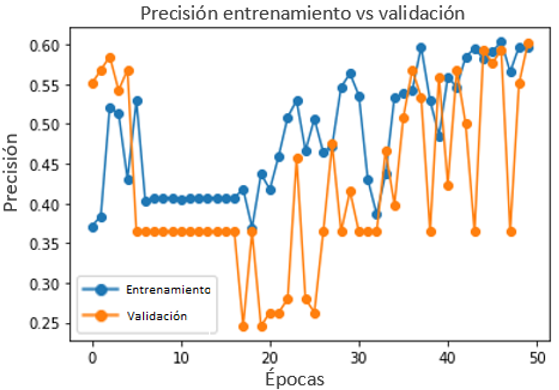
\includegraphics[scale=0.5]{Figs/101.png}
	\caption{Accuracy Modelo VGG19}
	\label{fig:VGG19_accuracy}
\end{figure}  

La precisión del modelo al completar 50 épocas es inferior al 60 \%.	En la Figura \ref{fig:VGG19_losses}, se puede apreciar que el modelo cuenta con \textit{16 \%} de desviación aproximadamente entre las predicciones y los valores reales, implementados durante el entrenamiento del modelo.

\begin{figure}[ht]
	\centering
	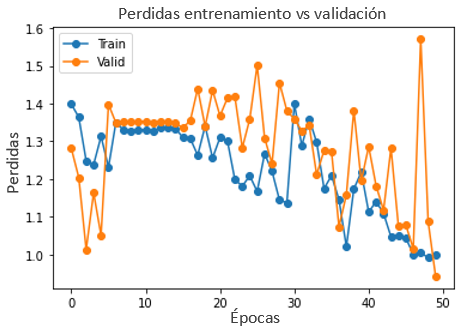
\includegraphics[scale=0.55]{Figs/102.png}
	\caption{Losses Modelo VGG19}
	\label{fig:VGG19_losses}
\end{figure}

Teniendo en cuenta la información presentada en las Figuras \ref{fig:VGG19_accuracy} y \ref{fig:VGG19_losses}, se puede apreciar que el modelo presenta \textit{overfiting} durante el transcurso de las épocas 18 hasta la época 30, y finalmente culminada la época 50 del modelo, el porcentaje de \textit{overfiting} es aproximadamente cero, y se procede a presentar en la Figura \ref*{fig:VGG19_prediccion} la predicción realizada por el modelo.

\begin{figure}[ht]
	\centering
	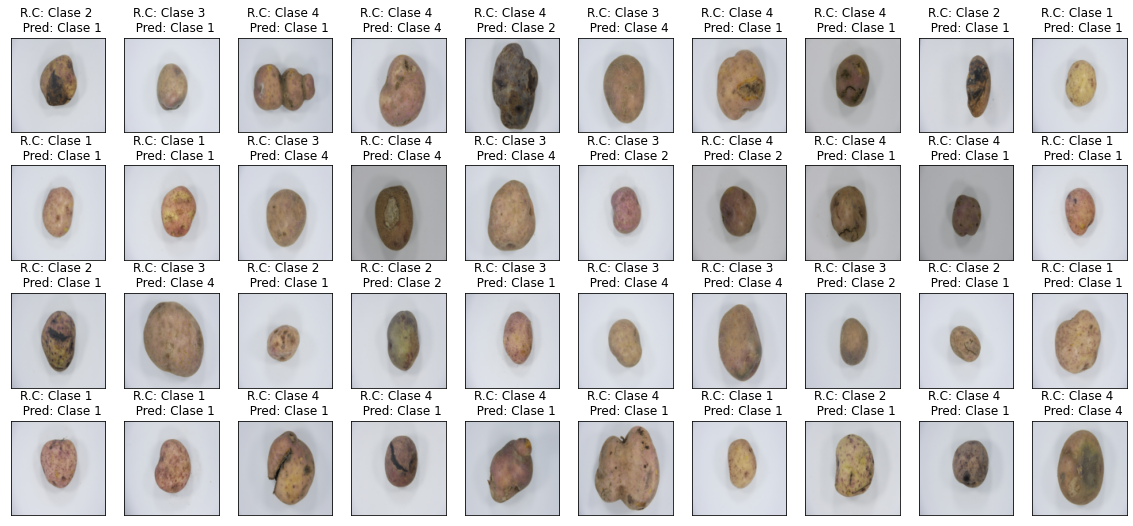
\includegraphics[scale=0.4]{Figs/103.png}
	\caption{Predicción Modelo VGG19}
	\label{fig:VGG19_prediccion}
\end{figure}

\newpage
Luego de esto see genera la matriz de confusión para validar los verdaderos positivos, verdaderos negativos, falsos positivos y falsos negativos, La Tabla \ref{fig:MC_VGG19} muestra los resultados.


\begin{table}[htbp]
	\centering
	\begin{tabular}{|c|l|c|c|c|c|}
		\hline
		\multicolumn{2}{|c|}{\multirow{2}[4]{*}{}} & \multicolumn{4}{c|}{Predicción} \bigstrut\\
		\cline{3-6}    \multicolumn{2}{|c|}{} & CLASE 1 & CLASE 2 & CLASE 3 & CLASE 4 \bigstrut\\
		\hline
		\multirow{4}[8]{*}{\begin{sideways}Observación\end{sideways}} & CLASE 1 & 27     & 2     & 0    & 0 \bigstrut\\
		\cline{2-6}     & CLASE 2 & 21     & 1     & 0    & 2 \bigstrut\\
		\cline{2-6}      & CLASE 3 & 6     & 5     & 0    & 11 \bigstrut\\
		\cline{2-6}     & CLASE 4 & 20     & 15     & 0    & 8 \bigstrut\\
		\hline
	\end{tabular}%
	\caption{Matriz de confusión modelo VGG-19}
	\label{fig:MC_VGG19}
\end{table}%

En la Tabla \ref{fig:ACU_VGG19}, se presenta la precisión del modelo VGG-19 obtenida en el entrenamiento, en cada una de las clases definidas.

\begin{table}[htbp]
	\centering
	\begin{tabular}{|c|c|}
		\hline
		CLASE 1 & 75.9 \bigstrut\\
		\hline
		CLASE 2 & 50 \bigstrut\\
		\hline
		CLASE 3 & 90.9 \bigstrut\\
		\hline
		CLASE 4 & 51.2 \bigstrut\\
		\hline
		\multicolumn{2}{|c|}{Overall Accuracy: 36.84210} \bigstrut\\
		\hline
	\end{tabular}%
	\caption{Precisión por clase modelo VGG19}
	\label{fig:ACU_VGG19}
\end{table}%


\newpage
\subsubsection{\MakeUppercase{Modelo preentrenado VGG11}}
VGG es un modelo preentrenado, en un conjunto de datos que contiene el peso que representan las características del conjunto de datos entrenados. Los modelos VGG toman una imagen de entrada de dimensiones \textit{224 x 224} pixeles en formato RGB, que son tratadas con un tamaño de imagen constante.\\


El modelo de aprendizaje profundo VGG11. Es la configuración más sencilla. Tiene 11 capas de peso en total, de ahí el nombre VGG-11, 8 de ellas son capas convolucionales y 3 son capas completamente conectadas, como se aprecia en la Figura \ref{fig:VGG11} \cite{ref_3}.

\begin{figure}[ht]
	\centering
	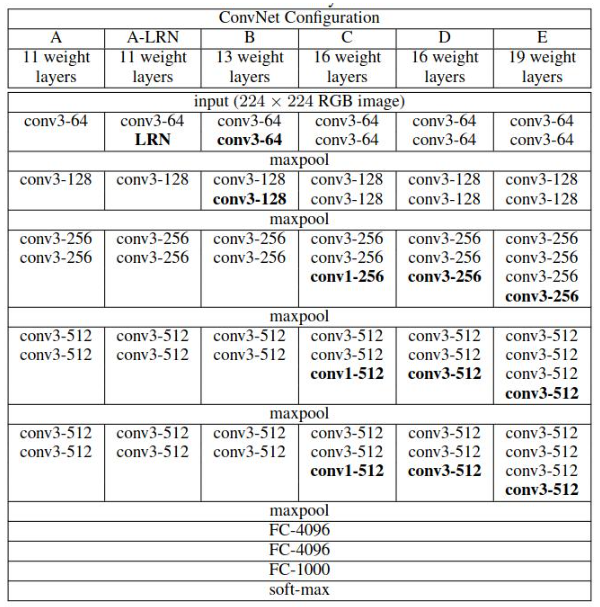
\includegraphics[scale=0.6]{Figs/70.png}
	\caption{Composición Modelo VGG-11}
	\label{fig:VGG11}
\end{figure}

Las 11 capas del modelo VGG11 son:
\begin{itemize}
	\item Convolución usando 64 filtros + Max Pooling
	\item Convolución usando 128 filtros + Max Pooling
	\item Convolución usando 256 filtros
	\item Convolución usando 256 filtros + Max Pooling
	\item Convolución usando filtros 512
	\item Convolución usando 512 filtros + Max Pooling
	\item Convolución usando filtros 512
	\item Convolución usando 512 filtros + Max Pooling
	\item Totalmente conectado con 4096 nodos
	\item Totalmente conectado con 4096 nodos
	\item Capa de salida con activación Softmax con 1000 nodos.
\end{itemize}

El modelo cuenta con 11 capas ponderadas, sus pesos representan la fuerza de las conexiones entre unidades de capas de red adyacentes, son implementadas con el fin de conectar cada neurona de una capa con todas las neuronas de la siguiente capa, se debe tener en cuenta que la capa MAX-POOLING no se considera como una capa ponderada, debido a que es un mapa de características que contiene las características más destacadas.\\

El Max-Pooling es una operación de pooling, que calcula el valor máximo que contiene cada parche en cada mapa de características, como resultado se obtienen mapas de características muestreados, que destacan la característica más relevante en el parche, en la practica se ha comprobado que este método, es más eficiente que la agrupación media en tareas de visión por ordenador, como la clasificación de imágenes.\\		 


Una vez conocida la forma en que se estructura el modelo VGG-11, se procede a evaluar su precisión antes de ser aplicada la optimización bayesiana y durante 50 épocas. La Figura \ref{fig:precision_VGG11}, muestra la precsión obtenida durante el entrenamiento, que no supera el 25 \%.


\begin{figure}[ht]
	\centering
	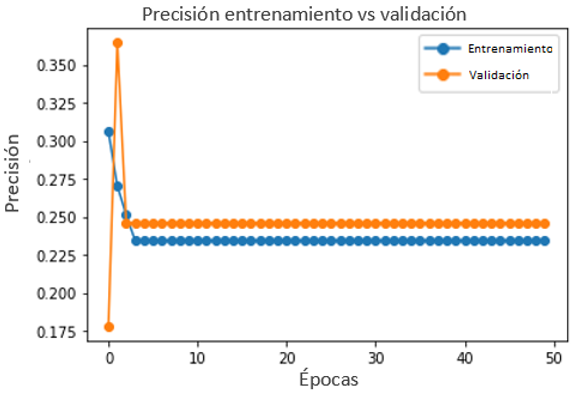
\includegraphics[scale=0.5]{Figs/105.png}
	\caption{Precisión Modelo VGG-11}
	\label{fig:precision_VGG11}
\end{figure}

En la Figura \ref{fig:loses_VGG11}, se aprecia que el modelo cuenta con una desviación bastante significativa, entre las predicciones y los valores reales. Gracias a la información brindada por las figuras anteriores se deduce que el sistema posee un alto porcentaje de \textit{overfiting}, que no puede ser corregido en el transcurso de las épocas.

\begin{figure}[ht]
	\centering
	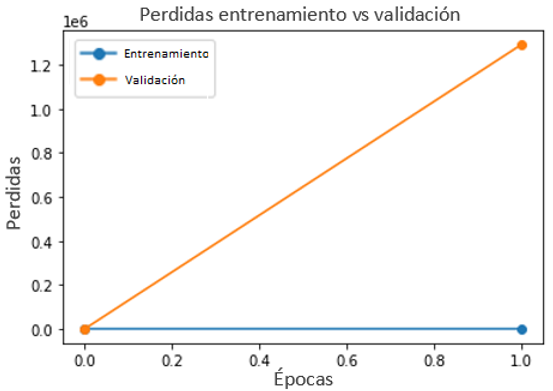
\includegraphics[scale=0.5]{Figs/106.png}
	\caption{Losses Modelo VGG-11}
	\label{fig:loses_VGG11}
\end{figure}

En la Figra \ref{fig:Pre_VGG11}, se presenta la predicción del modelo VGG-11 con las muestras implementadas para su validación.

\begin{figure}[ht]
	\centering
	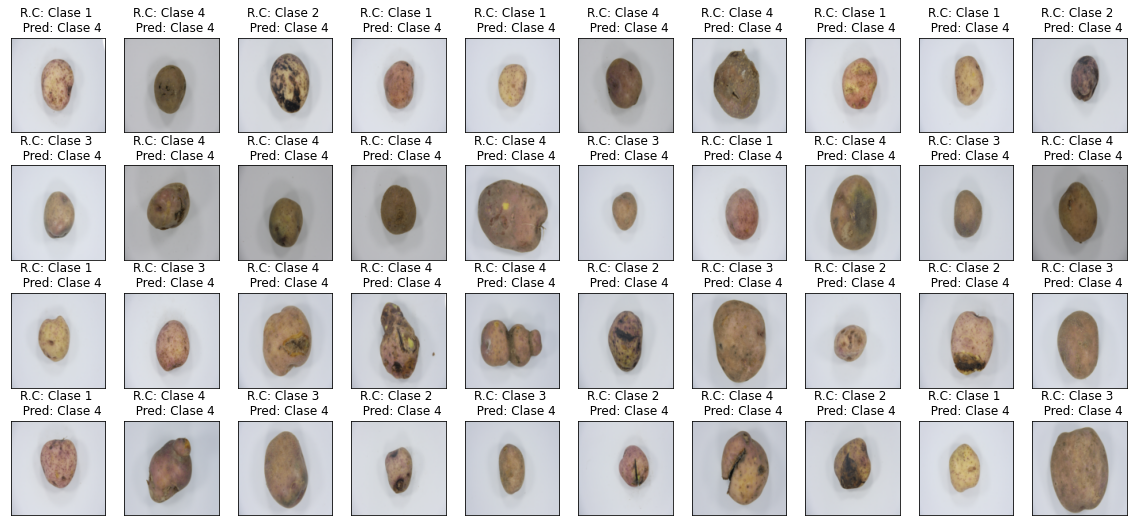
\includegraphics[scale=0.4]{Figs/107.png}
	\caption{Predicción Modelo VGG-11}
	\label{fig:Pre_VGG11}
\end{figure}

La Tabla \ref{fig:MC_VGG11}, presenta la matriz de confusión del modelo VGG-11, donde se aprecian los verdaderos positivos, verdaderos negativos, falsos positivos y falsos negativos.

\newpage
\begin{table}[htbp]
	\centering
	\begin{tabular}{|c|l|c|c|c|c|}
		\hline
		\multicolumn{2}{|c|}{\multirow{2}[4]{*}{}} & \multicolumn{4}{c|}{Predicción} \bigstrut\\
		\cline{3-6}    \multicolumn{2}{|c|}{} & CLASE 1 & CLASE 2 & CLASE 3 & CLASE 4 \bigstrut\\
		\hline
		\multirow{4}[8]{*}{\begin{sideways}Observación\end{sideways}} & CLASE 1 & 0     & 0     & 0    & 29 \bigstrut\\
		\cline{2-6}     & CLASE 2 & 0     & 0     & 0    & 24 \bigstrut\\
		\cline{2-6}      & CLASE 3 & 0     & 0     & 0    & 22 \bigstrut\\
		\cline{2-6}     & CLASE 4 & 0     & 0     & 0    & 43 \bigstrut\\
		\hline
	\end{tabular}%
	\caption{Matriz de confusión VGG-11}
	\label{fig:MC_VGG11}
\end{table}%

Finalmente, se obtiene la precisión de clasificación del modelo VGG-11 por clases en la Tabla \ref{fig:clase_VGG11}.

\begin{table}[ht]
	\centering
	\begin{tabular}{|c|c|}
		\hline
		CLASE 1 & 0 \bigstrut\\
		\hline
		CLASE 2 & 0 \bigstrut\\
		\hline
		CLASE 3 & 0 \bigstrut\\
		\hline
		CLASE 4 & 100 \bigstrut\\
		\hline
		\multicolumn{2}{|c|}{Overall Accuracy: 34.21052} \bigstrut\\
		\hline
	\end{tabular}%
	\caption{Clasificación por clase modelos VGG-11}
	\label{fig:clase_VGG11}
\end{table}%  


\newpage
\subsubsection{\MakeUppercase{Modelo preentrenado RESNET18}}
La arquitectura Resnet, (Residual Net), fue propuesta por un equipo de Microsoft Research, el cual fue liderado por Kaiming He, en donde se propone que si a una red neuronal de 20 capas, se le intercalan 36 capas que calculan la simple función de identidad, la red resultante, (56 capas), debería tener exactamente la misma eficacia y no ser inferior que la primera. Se debe recordar que la función identidad es la encargada de devolver exactamente el mismo valor que su argumento \cite{ref_4}.\\

Conociendo esto para permitir que una red pueda variar su cantidad efectiva de capas, se introduce el concepto de bloque residual:

\begin{figure}[ht]
	\centering
	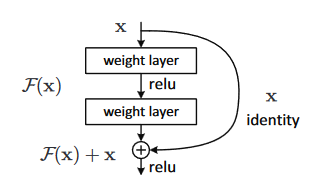
\includegraphics[scale=0.6]{Figs/67.png}
	\caption{Bloque Residual}
	\label{fig:Bloque}
\end{figure}

Como se aprecia en la Figura \ref{fig:Bloque}, el bloque residual se compone de una ruta residual, (izquierda), y una conexión atajo, (derecha), que la soslaya. La ruta residual F(x), esta compuesta de dos capas de pesos sinapticos, (pueden ser densas o convolucionales), que se intercalan por una función rectificadora. El resultado se suma con la información que atraviesa la conexión atajo \textit{X "identidad"}. Y por ultimo se aplica nuevamente la función rectificadora. La información puede atravesar con ello dos caminos diferentes que son: el de la función de identidad X o el de la ruta residual \textit{F(x)} \cite{ref_5}.

\newpage
En la arquitectura Resnet18, Las 18 capas de esta arquitectura representan las 18 capas con pesos, en donde se incluye la capa de convolución y la capa totalmente conectada, excluyendo la capa de agrupación y la capa BN.

\begin{figure}[ht]
	\centering
	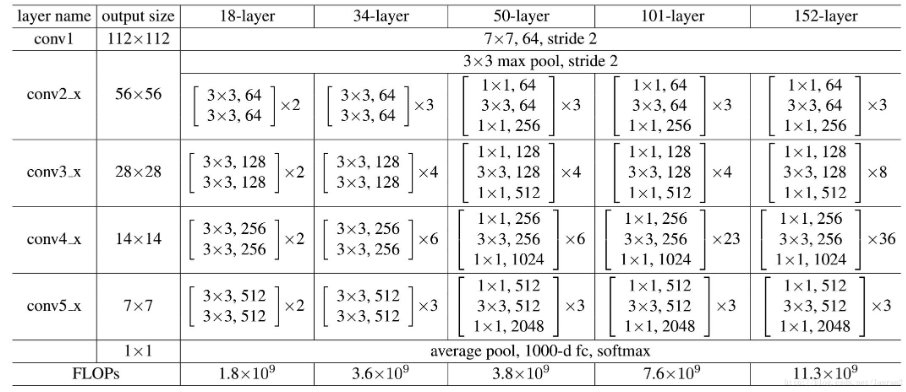
\includegraphics[scale=0.65]{Figs/68.png}
	\caption{Arquitectura ResNet18}
	\label{fig:ArqRes18}
\end{figure}


Como se puede observar en la Figura \ref{fig:ArqRes18}, la primera capa de convolución implementa una plantilla de \textit{7 x 77 x 7}, con un tamaño de paso de 2 y un relleno de 3, Seguido a eso, se realiza BN, ReLu y Maxpooling. Estos constituyen la primera parte del modulo de convolucion conv1.\\

Luego hay cuatro etapas, cada etapa tiene múltiples módulos, cada módulo se llama un bloque de construcción, por ende se evidencia que hay 8 bloques de construcción, como se presenta en la Figura \ref{fig:ArqRes18} \cite{ref_5}.				


\newpage	
En la Figura \ref{fig:preci_RESNET18}, se procede a presentar la precisión obtenida del modelo ResNet-18 durante 50 épocas, sin haber aplicado la optimizacion bayesiana.

\begin{figure}[ht]
	\centering
	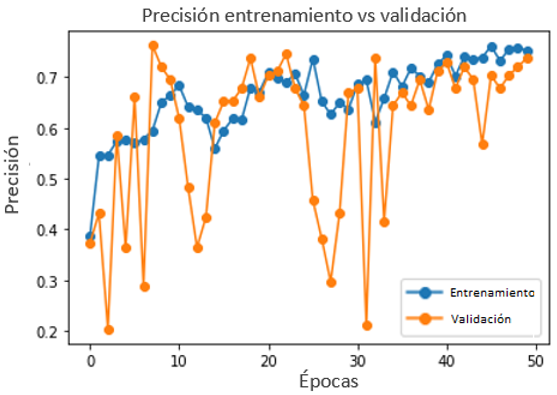
\includegraphics[scale=0.55]{Figs/109.png}
	\caption{Precisión modelo Resnet-18}
	\label{fig:preci_RESNET18}
\end{figure}

La información presentada en la Figura \ref{fig:perdda_RESNET18}, permite observar que el modelo cuenta con una desviación muy baja entre las predicciones y los valores reales, permitiendo concluir que el modelo cuenta con un bajo porcentaje de \textit{overfiting}. 

\begin{figure}[ht]
	\centering
	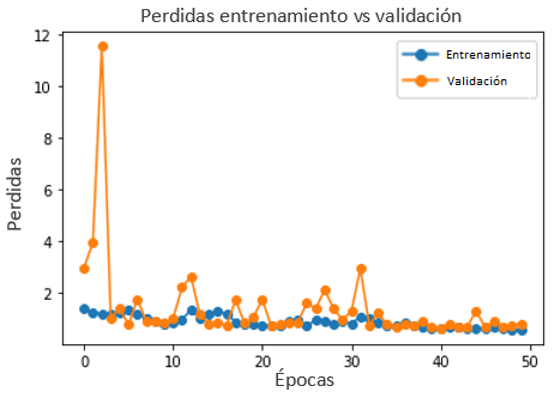
\includegraphics[scale=0.55]{Figs/110.png}
	\caption{Perdidas modelo Resnet-18}
	\label{fig:perdda_RESNET18}
\end{figure}

\newpage
La Figura \ref{fig:pre_RESNET18}, presenta las predicciones realizadas por el modelo ResNet-18 con las muestras implementadas durante su validación.

\begin{figure}[ht]
	\centering
	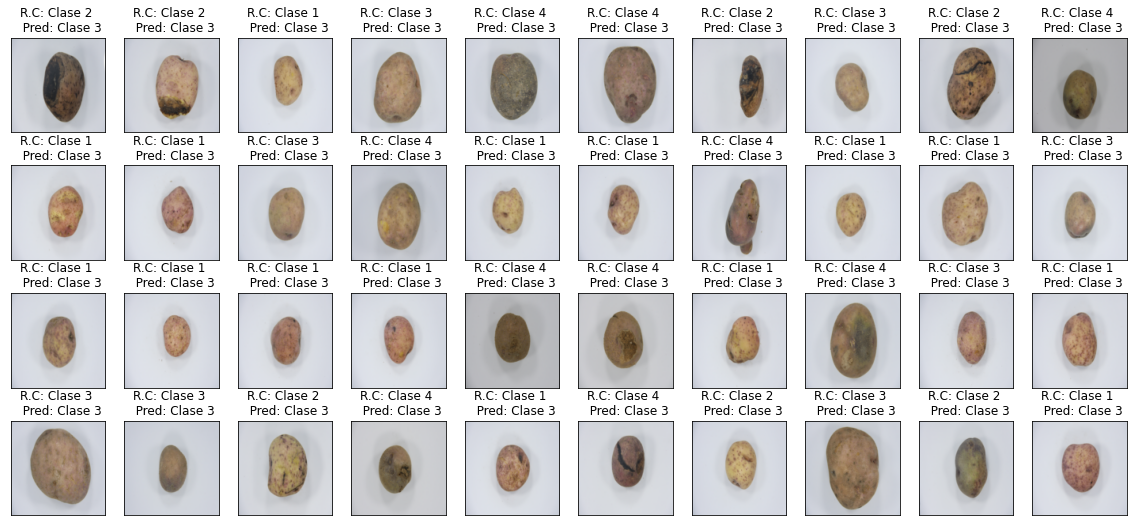
\includegraphics[scale=0.4]{Figs/111.png}
	\caption{Predicción modelo Resnet-18}
	\label{fig:pre_RESNET18}
\end{figure}

La matriz de confusión del modelos ResNet-18 es presentada en la Tabla \ref*{MC_RESNET18} , con el fin de dar a conocer los verdaderos positivos, verdaderos negativos, falsos positivos, y falsos negativos del modelo

\begin{table}[htbp]
	\centering
	\begin{tabular}{|c|l|c|c|c|c|}
		\hline
		\multicolumn{2}{|c|}{\multirow{2}[4]{*}{}} & \multicolumn{4}{c|}{Predicción} \bigstrut\\
		\cline{3-6}    \multicolumn{2}{|c|}{} & CLASE 1 & CLASE 2 & CLASE 3 & CLASE 4 \bigstrut\\
		\hline
		\multirow{4}[8]{*}{\begin{sideways}Observación\end{sideways}} & CLASE 1 & 0     & 0     & 29    & 0 \bigstrut\\
		\cline{2-6}          & CLASE 2 & 0     & 0     & 24    & 0 \bigstrut\\
		\cline{2-6}          & CLASE 3 & 0     & 0     & 22    & 0 \bigstrut\\
		\cline{2-6}          & CLASE 4 & 0     & 0     & 43    & 0 \bigstrut\\
		\hline
	\end{tabular}%
	\caption{Matriz de confusión ResNet-18}
	\label{MC_RESNET18}
\end{table}%

Para finalizar, en la Tabla \ref*{clase_RESNET18}, se presenta la precisión del modelo sin optimización bayesiana por clases.

\begin{table}[htbp]
	\centering
	\begin{tabular}{|c|c|}
		\hline
		CLASE 1 & 0 \bigstrut\\
		\hline
		CLASE 2 & 0 \bigstrut\\
		\hline
		CLASE 3 & 100 \bigstrut\\
		\hline
		CLASE 4 & 0 \bigstrut\\
		\hline
		\multicolumn{2}{|c|}{Overall Accuracy: 18,42105} \bigstrut\\
		\hline
	\end{tabular}%
	\caption{Clasificación por clase modelos ResNet-18}
	\label{clase_RESNET18}
\end{table}%


\newpage	
\subsubsection{\MakeUppercase{Comparación de arquitecturas sin optimizar}}
En la Tabla \ref{table:compasin}, se presenta la comparación de los cuatro modelos sin optimización bayesiana, implementados para la clasificación de tubérculos de papa.

\begin{table}[ht]
	\centering
	\begin{tabular}{|c|c|c|c|c|}
		\hline
		MODELOS & AlexNet & VGG-19 & VGG-11 & ResNet-18 \\
		\hline
		PRECISIÓN (\%) &  & $$36.84$$ & $$34.21$$ & $$18.42$$ \\
		\hline
		PERDIDAS (\%) &  & $$16$$ & $$12$$ & $$2$$ \\
		\hline
	\end{tabular}	
	\caption{Comparación modelos sin optimizar}
	\label{table:compasin}
\end{table}	

En la Tabla \ref{table:compasin},se puede observar que el modelo con mejor precisión es el modelo \textit{VGG-19}, esto debido a que la función de perdidas de este modelo no presenta una desviación significativa entre los valores predichos y los valores reales implementados. El modelo AlexNet no es tenido en cuenta, ya que este modelo presento una precisión por debajo del 10 \% tanto en la etapa del entrenamiento como en la etapa de validación.


\newpage
\subsection{Optimización Bayesiana}

Dos de las estrategias más empleadas para probar diferentes combinaciones de hipérparámetros y evaluarlas mediante métodos de validación, son \textit{grid search y random search} \cite{liashchynskyi2019grid}. En la primera estrategia, los valores estudiados de cada hiperparámetro, son distribuidos uniformemente dentro de un rango delimitado por el analista. En la segunda estrategia, los datos son aleatorios dentro de ese rango como se muestra en la Figura \ref{fig:Hiperparámetros grid search y random search}.

\begin{figure}[ht]
	\centering
	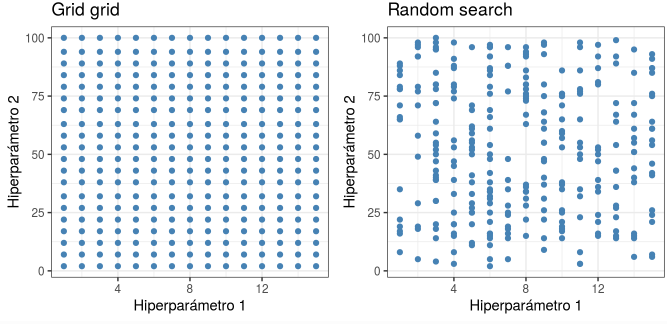
\includegraphics[scale=0.6]{Figs/121.png}
	\caption{Métodos de Optimización De Hiperparámetros}
	\label{fig:Hiperparámetros grid search y random search}
\end{figure}

A pesar de que las dos estrategias son válidas y se obtienen buenos resultados, sobretodo cuando se tiene criterio para acotar el rango de búsqueda, poseen una carencia similar: ninguna de las dos tiene en cuenta los resultados obtenidos hasta el momento, lo cual impide que se focalicen en la búsqueda de las regiones de mayor interés y evitando las regiones innecesarias.\\


Otro método utilizado para la búsqueda de los hiperparámetros de un modelo, es la optimización bayesiana, la cual consiste en crear un modelo probabilístico, en el que el valor de la función objetivo es la métrica de validación del modelo, en este caso, la presición. Con este método, se logra que la búsqueda se vaya redirigiendo en cada iteración hacia las regiones de mayor interés \cite{frazier2018tutorial}. Esto con el fin de reducir el número de combinaciones de los hiperparámetros con los que el modelo es evaluado, seleccionando únicamente los mejores candidatos. Esto significa que, la ventaja frente a las estrategias descritas anteriormente, se maximiza cuando el espacio de búsqueda es muy amplio o la evaluación del modelo es muy lenta.\\

Para realizar la optimización bayesiana, se utilizó el módulo para \textit{Python} \textit{Botorch}  \cite{balandat2020botorch}. Es el motor de optimización de \textit{Ax-Services} compatible con \textit{Pytorch}, que admite algunas funciones de minimización y maximización, como la mejora esperada (\textit{EI}), la probabilidad de mejora y el límite superior de confianza. La mejora esperada es una función de adquisición recompensa la evaluación del objetivo $f$, basándose en la mejora esperada en relación con el mejor momento. En la Ecuación \ref{EI} se define  \textit{EI} .

\begin{equation}
	{EI(x)=\in[max(f(x)-f*),0]}
	\label{EI}
\end{equation}

El resultado de la parametrización, con la mejora esperada, se selecciona y se evalúa en el siguiente paso. Una vez que se ha explorado adecuadamente el espacio de los parámetros, la mejora esperada se estrecha naturalmente en las ubicaciones donde hay una alta probabilidad de un buen valor objetivo. Este proceso se realiza por 20 etapas de acuerdo a los parámetros de optimización elegidos. La Tabla \ref{paraopt} muestra los parámetros escogidos para optimizar.

\begin{table}[ht]
	\centering
	\begin{tabular}{|c|c|c|ll}
		\cline{1-3}
		Parámetro & Limite inferior              & Limite Superior &  &  \\ \cline{1-3}
		lr         & $1*10^{-6}$ & 0.4             &  &  \\ \cline{1-3}
		Momentum   & 0                            & 1               &  &  \\ \cline{1-3}
		Stepsize   & 20                           & 40              &  &  \\ \cline{1-3}
	\end{tabular}
	\caption{Hiperparámetros Optimizados}
	\label{paraopt}
\end{table}

\textit{Botorch} realiza $20$ pruebas con parámetros distintos en los rangos definidos, y encuentra la combinación de parámetros que den el mejor resultado de precisión final del algoritmo. Estos resultados fueron utilizados para entrenar nuevamente los modelos descritos anteriormente. 




\newpage	
\subsubsection{\MakeUppercase{Modelo preentrenado AlexNet optimizado}}
En la Figura \ref{fig:preci_Alex_OPT}, se puede observar que el modelo AlexNet, implementando la optimización bayesiana, presenta un deterioro en la precisión cuando se realiza la validación.
\begin{figure}[ht]
	\centering
	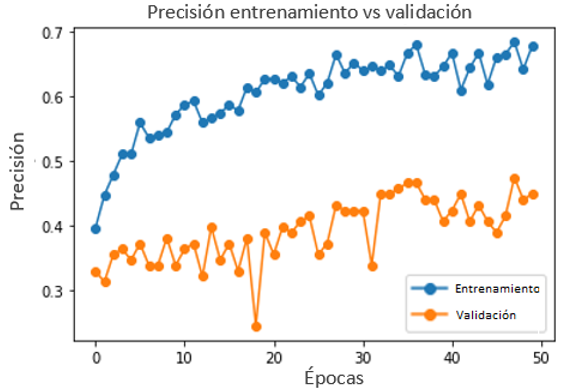
\includegraphics[scale=0.8]{Figs/500.png}
	\caption{Precisión modelo AlexNet optimizado}
	\label{fig:preci_Alex_OPT}
\end{figure}

En la Figura \ref{fig:perdda_Alex_opt}, se aprecia que el modelo AlexNet es poco eficiente, ya que existe una desviación significativa entre la predicción realizada y los valores reales implementados.
\begin{figure}[ht]
	\centering
	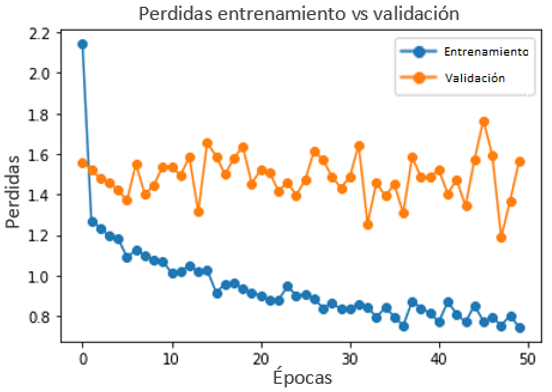
\includegraphics[scale=0.8]{Figs/501.png}
	\caption{Perdidas modelo AlexNet optimizado}
	\label{fig:perdda_Alex_opt}
\end{figure}

\newpage
La Figura \ref{fig:pre_alex_opt}, presenta la clasificación realizada por el modelo con las muestras implementadas.
\begin{figure}[ht]
	\centering
	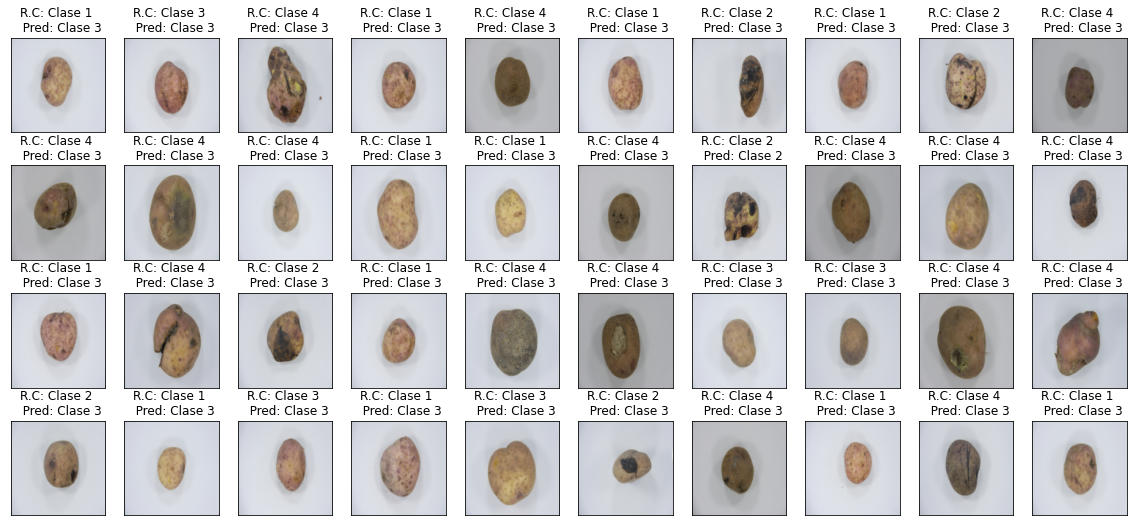
\includegraphics[scale=0.4]{Figs/502.png}
	\caption{Predicción modelo AlexNet optimizado}
	\label{fig:pre_alex_opt}
\end{figure}


La Tabla \ref{tab:MC_ALEX_OPT}, almacena los datos de la matriz de confusión del modelo AlexNet, esto con el fin de dar a conocer los verdaderos positivos, verdaderos negativos, falsos positivos y falsos negativos del modelo.


\begin{table}[htbp]
	\centering
	\begin{tabular}{|c|l|c|c|c|c|}
		\hline
		\multicolumn{2}{|c|}{\multirow{2}[4]{*}{}} & \multicolumn{4}{c|}{Predicción} \bigstrut\\
		\cline{3-6}    \multicolumn{2}{|c|}{} & CLASE 1 & CLASE 2 & CLASE 3 & CLASE 4 \bigstrut\\
		\hline
		\multirow{4}[8]{*}{\begin{sideways}Observación\end{sideways}} & CLASE 1 & 0     & 0     & 29    & 0 \bigstrut\\
		\cline{2-6}          & CLASE 2 & 0     & 1     & 22    & 1 \bigstrut\\
		\cline{2-6}          & CLASE 3 & 0     & 0     & 22    & 0 \bigstrut\\
		\cline{2-6}          & CLASE 4 & 0     & 1     & 42    & 0 \bigstrut\\
		\hline
	\end{tabular}%
	\caption{Matriz de confusión AlexNet Optimizado }
	\label{tab:MC_ALEX_OPT}%
\end{table}%

\newpage
Para finalizar, en la Tabla \ref{tab:Alexoptclases} se presenta la precisión del modelo por cada clase de clasificación y la precisión general.

\begin{table}[htbp]
	\centering
	\begin{tabular}{|c|c|}
		\hline
		CLASE 1 & 0 \bigstrut\\
		\hline
		CLASE 2 & 4.2 \bigstrut\\
		\hline
		CLASE 3 & 100 \bigstrut\\
		\hline
		CLASE 4 & 0 \bigstrut\\
		\hline
		\multicolumn{2}{|c|}{Overall Accuracy: 21,05263} \bigstrut\\
		\hline
	\end{tabular}%
	\caption{Clasificación por clase modelos AlexNet}
	\label{tab:Alexoptclases}%
\end{table}%


\newpage
\subsubsection{\MakeUppercase{Modelo preentrenado VGG-19 optimizado}}
La Figura \ref{fig:preci_vgg19_OPT}, muestra que la precisión del modelo VGG-19 es de alrededor del 75 \% en validación, el cual es un valor que se acerca mucho al valor del modelo en entrenamiento, el cual era de aproximadamente el 80 \%.
\begin{figure}[ht]
	\centering
	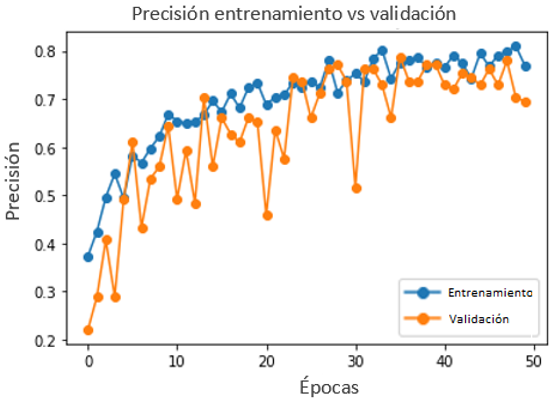
\includegraphics[scale=0.6]{Figs/504.png}
	\caption{Precisión modelo VGG-19 optimizado}
	\label{fig:preci_vgg19_OPT}
\end{figure}

La Figura \ref{fig:perdda_vgg19_opt}, permite verificar que el modelo VGG-19 es bueno, ya que la desviación que existe entre la prediccón realizada y los valores reales implementados es muy baja.


\begin{figure}[ht]
	\centering
	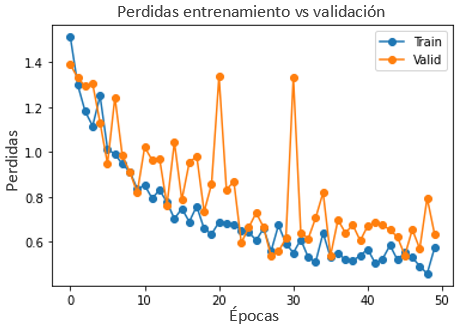
\includegraphics[scale=0.6]{Figs/505.png}
	\caption{Perdidas modelo VGG-19 optimizado}
	\label{fig:perdda_vgg19_opt}
\end{figure}

\newpage
Se puede apreciar la clasificación y eficiencia del modelo en la Figura \ref{fig:pre_vgg19_opt}.

\begin{figure}[ht]
	\centering
	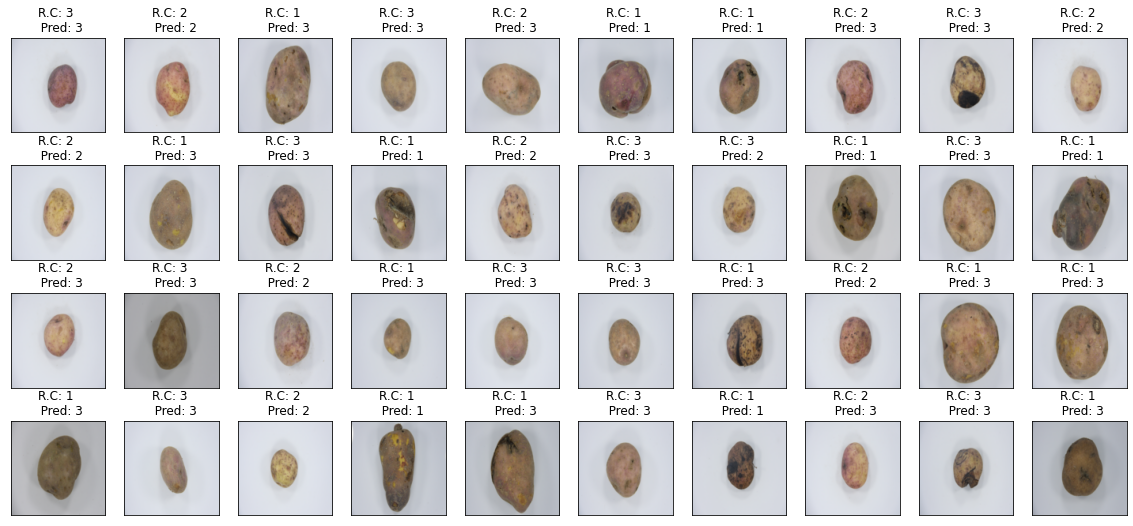
\includegraphics[scale=0.4]{Figs/506.png}
	\caption{Predicción modelo VGG-19 optimizado}
	\label{fig:pre_vgg19_opt}
\end{figure}

En la Tabla \ref{tab:MC_VGG19_OPT}, se presenta la matriz de confusión del modelo VGG-19, la cual es necesaria para tener conocimiento de los verdaderos positivos, verdaderos negativos, falsos positivos y falsos negativos que presenta el modelo.

\begin{table}[htbp]
	\centering
	\begin{tabular}{|c|l|c|c|c|c|}
		\hline
		\multicolumn{2}{|c|}{\multirow{2}[4]{*}{}} & \multicolumn{4}{c|}{Predicción} \bigstrut\\
		\cline{3-6}    \multicolumn{2}{|c|}{} & CLASE 1 & CLASE 2 & CLASE 3 & CLASE 4 \bigstrut\\
		\hline
		\multirow{4}[8]{*}{\begin{sideways}Observación\end{sideways}} & CLASE 1 & 22    & 0     & 7    & 0 \bigstrut\\
		\cline{2-6}          & CLASE 2 & 4     & 12     & 1    & 7 \bigstrut\\
		\cline{2-6}          & CLASE 3 & 1     & 0     & 20    & 1 \bigstrut\\
		\cline{2-6}          & CLASE 4 & 1     & 1     & 19    & 22 \bigstrut\\
		\hline
	\end{tabular}%
	\caption{Matriz de confusión VGG-19 Optimizado }
	\label{tab:MC_VGG19_OPT}%
\end{table}%


\newpage
Para finalizar, en la Tabla \ref{tab:VGG19optclases}, se presentan las precisiones realizadas por el modelo para cada clase a clasificar y la precisión en general.
\begin{table}[htbp]
	\centering
	\begin{tabular}{|c|c|}
		\hline
		CLASE 1 & 75.9 \bigstrut\\
		\hline
		CLASE 2 & 50 \bigstrut\\
		\hline
		CLASE 3 & 90.9 \bigstrut\\
		\hline
		CLASE 4 & 51.2 \bigstrut\\
		\hline
		\multicolumn{2}{|c|}{Overall Accuracy: 65.78947} \bigstrut\\
		\hline
	\end{tabular}%
	\caption{Clasificación por clase modelos VGG-19}
	\label{tab:VGG19optclases}%
\end{table}%

\subsubsection{\MakeUppercase{Modelo preentrenado VGG-11 optimizado}}
En la Figura \ref{fig:preci_vgg11_OPT}, se puede observar que la precisión del modelo VGG-11 cuando se valida, es cercana a la precisión obtenida cuando el modelo es entrenado.

\begin{figure}[ht]
	\centering
	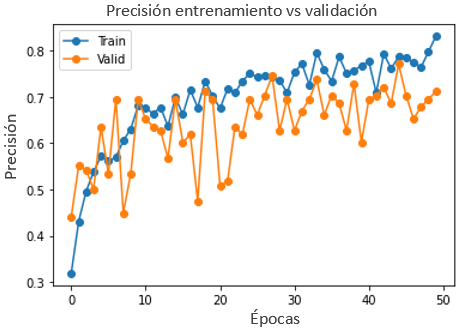
\includegraphics[scale=0.6]{Figs/508.png}
	\caption{Precisión modelo VGG-11 optimizado}
	\label{fig:preci_vgg11_OPT}
\end{figure}

La Figura \ref{fig:perdda_vgg11_opt}, permite apreciar que apesar que en el modelo existe una clara desviación en cuanto a los datos predichos y los valores reales implementados, esta no es lo suficientemente grande para convertir al modelo en ineficiente.

\newpage
\begin{figure}[ht]
	\centering
	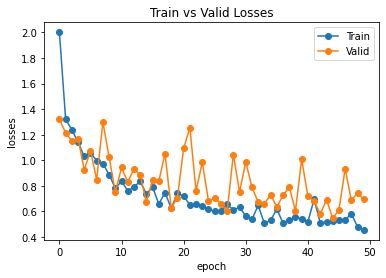
\includegraphics[scale=0.6]{Figs/509.png}
	\caption{Perdidas modelo VGG-11 optimizado}
	\label{fig:perdda_vgg11_opt}
\end{figure}


La Figura \ref{fig:pre_vgg11_opt}, permite evidenciar la precisión y eficiencia del modelo al clasificar los tubérculos de papas implementados. 	
\begin{figure}[ht]
	\centering
	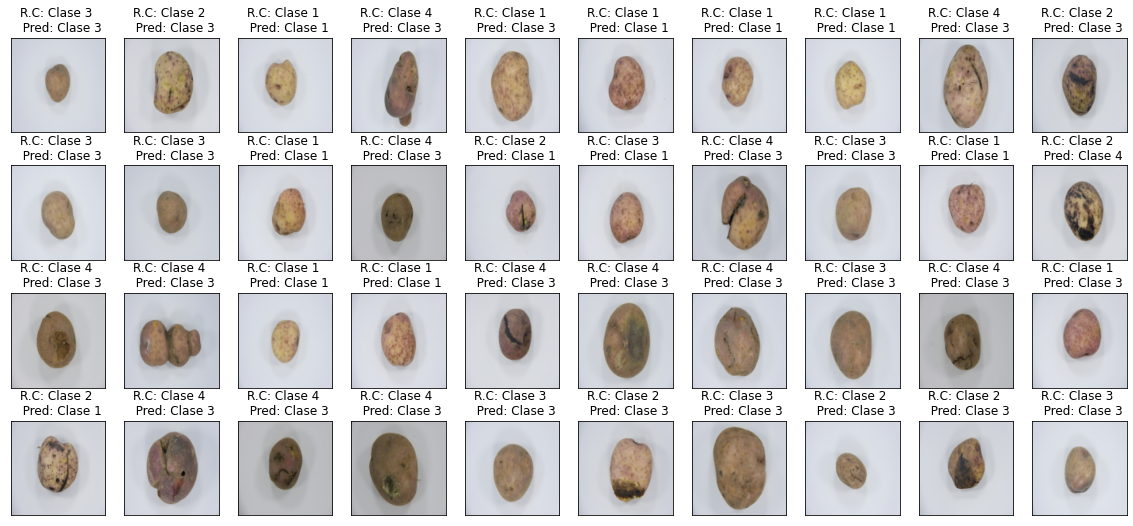
\includegraphics[scale=0.4]{Figs/510.png}
	\caption{Predicción modelo VGG-11 optimizado}
	\label{fig:pre_vgg11_opt}
\end{figure}

\newpage
La Tabla \ref{tab:MC_VGG11_OPT}, almacena la matriz de confusión del modelo VGG-11, la cual da a conocer los verdaderos positivos, verdaderos negativos, falsos positivos y falsos negativos que presenta el modelo.
\begin{table}[htbp]
	\centering
	\begin{tabular}{|c|l|c|c|c|c|}
		\hline
		\multicolumn{2}{|c|}{\multirow{2}[4]{*}{}} & \multicolumn{4}{c|}{Predicción} \bigstrut\\
		\cline{3-6}    \multicolumn{2}{|c|}{} & CLASE 1 & CLASE 2 & CLASE 3 & CLASE 4 \bigstrut\\
		\hline
		\multirow{4}[8]{*}{\begin{sideways}Observación\end{sideways}} & CLASE 1 & 18     & 0     & 11    & 0 \bigstrut\\
		\cline{2-6}          & CLASE 2 & 4     & 0     & 18    & 2 \bigstrut\\
		\cline{2-6}          & CLASE 3 & 2     & 0     & 20    & 0 \bigstrut\\
		\cline{2-6}          & CLASE 4 & 1     & 0     & 41    & 1 \bigstrut\\
		\hline
	\end{tabular}%
	\caption{Matriz de confusión VGG-11 Optimizado }
	\label{tab:MC_VGG11_OPT}%
\end{table}%

Por ultimo, en la Tabla \ref{tab:VGG11optclases}, se presentan las precisiones realizadas por el modelo para cada clase a clasificar y la precisión en general.

\begin{table}[htbp]
	\centering
	\begin{tabular}{|c|c|}
		\hline
		CLASE 1 & 62.1 \bigstrut\\
		\hline
		CLASE 2 & 0 \bigstrut\\
		\hline
		CLASE 3 & 90.9 \bigstrut\\
		\hline
		CLASE 4 & 2.3 \bigstrut\\
		\hline
		\multicolumn{2}{|c|}{Overall Accuracy: 39,47368} \bigstrut\\
		\hline
	\end{tabular}%
	\caption{Clasificación por clase modelos VGG-11}
	\label{tab:VGG11optclases}%
\end{table}%

\newpage	
\subsubsection{\MakeUppercase{Modelo Preentrenado ResNet-18 Optimizado}}

La precisión del modelos ResNet-18 se presenta en la Figura \ref{fig:preci_RES_OPT}, en donde se puede apreciar que el modelo, tiene un gran margen de error en su validación con respecto a la precisión obtenida durante su entrenamiento.

\begin{figure}[ht]
	\centering
	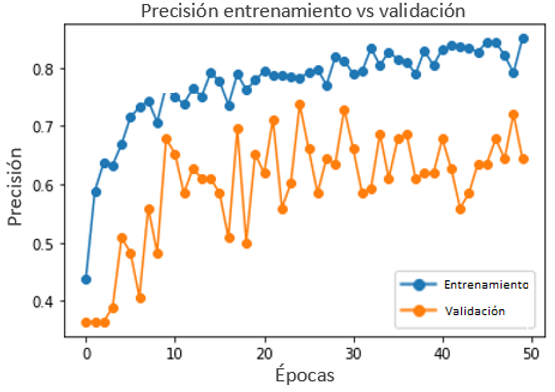
\includegraphics[scale=0.6]{Figs/512.png}
	\caption{Precisión modelo ResNet-18 optimizado}
	\label{fig:preci_RES_OPT}
\end{figure}

La Figura \ref{fig:perdda_REs_opt}, da a conocer que el modelo presenta overffiting, causando una desviación entre las predicciones realizadas y los datos reales implementados, volviendo así, poco eficiente el modelo.	

\begin{figure}[ht]
	\centering
	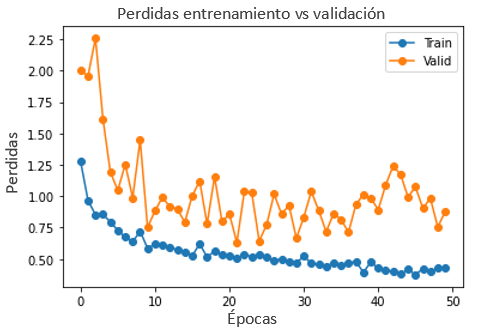
\includegraphics[scale=0.6]{Figs/513.png}
	\caption{Perdidas modelo ResNet-18 optimizado}
	\label{fig:perdda_REs_opt}
\end{figure}

\newpage
La Figura \ref{fig:pre_res_opt}, enseña la clasificación de los tubérculos implementados, realizada por el modelo ResNet-18.

\begin{figure}[ht]
	\centering
	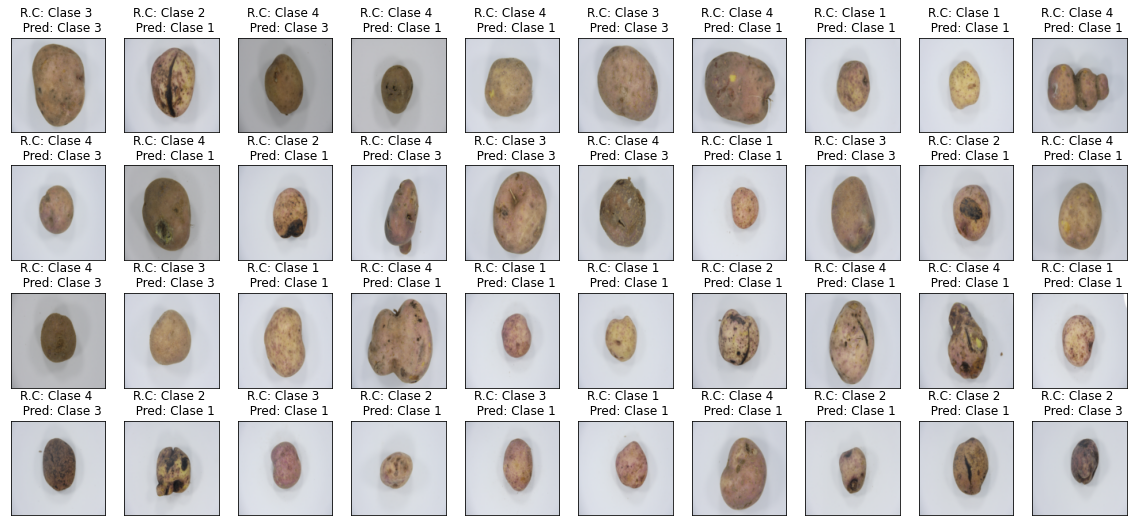
\includegraphics[scale=0.4]{Figs/514.png}
	\caption{Predicción modelo ResNet-18 optimizado}
	\label{fig:pre_res_opt}
\end{figure}

En la Tabla \ref{tab:MC_resnet_OPT}, se puede evidenciar la matriz de confusión del modelo ResNet-18, esto con el fin de conocer los verdaderos positivos, verdaderos negativos, falsos positivos y falsos negativos que se encuentran presentes en el modelo.

\begin{table}[htbp]
	\centering
	\begin{tabular}{|c|l|c|c|c|c|}
		\hline
		\multicolumn{2}{|c|}{\multirow{2}[4]{*}{}} & \multicolumn{4}{c|}{Predicción} \bigstrut\\
		\cline{3-6}    \multicolumn{2}{|c|}{} & CLASE 1 & CLASE 2 & CLASE 3 & CLASE 4 \bigstrut\\
		\hline
		\multirow{4}[8]{*}{\begin{sideways}Observación\end{sideways}} & CLASE 1 & 29     & 0     & 0    & 0 \bigstrut\\
		\cline{2-6}          & CLASE 2 & 19     & 0     & 5    & 0 \bigstrut\\
		\cline{2-6}          & CLASE 3 & 12     & 0     & 10    & 0 \bigstrut\\
		\cline{2-6}          & CLASE 4 & 21     & 0     & 21    & 1 \bigstrut\\
		\hline
	\end{tabular}%
	\caption{Matriz de confusión ResNet-18 Optimizado }
	\label{tab:MC_resnet_OPT}%
\end{table}%
Para finalizar, en la Tabla \ref{tab:resnetoptclases}, se presenta la precisión general del modelo ResNet-18 y la precisón por cada clase de clasificación.
\begin{table}[htbp]
	\centering
	\begin{tabular}{|c|c|}
		\hline
		CLASE 1 & 100 \bigstrut\\
		\hline
		CLASE 2 & 0 \bigstrut\\
		\hline
		CLASE 3 & 45.5 \bigstrut\\
		\hline
		CLASE 4 & 2.3 \bigstrut\\
		\hline
		\multicolumn{2}{|c|}{Overall Accuracy: 36,84210} \bigstrut\\
		\hline
	\end{tabular}%
	\caption{Clasificación por clase modelos ResNet-18}
	\label{tab:resnetoptclases}%
\end{table}%


\subsubsection{\MakeUppercase{Comparación de Arquitecturas Optimizadas}}

En la Tabla \ref{table:compacon}, se presenta la comparación de los cuatro modelos explicados anteriormente, aplicando optimización bayesiana con el objetivo de mejorar su precisión.

\begin{table}[ht]
	\centering
	\begin{tabular}{|c|c|c|c|c|}
		\hline
		MODELOS & AlexNet & VGG-19 & VGG-11 & ResNet-18 \\
		\hline
		PRECISIÓN (\%) & $$21.05$$ & $$65.78$$ & $$39.47$$ & $$36.84$$ \\
		\hline
		PERDIDAS (\%) & $$18$$ & $$16$$ & $$12$$ & $$65$$ \\
		\hline
	\end{tabular}	
	\caption{Comparación modelos optimizados}
	\label{table:compacon}
\end{table}	

En la Tabla \ref{table:compacon}, se puede observar que el modelo con mejor precisión es el modelo \textit{VGG-19}, pero también se aprecia que es el modelo con mayores perdidas. Sin embargo, se puede apreciar que la precisión de los modelos documentada en la Tabla \ref{table:compacon}, es superior a la precisión documentada en la Tabla \ref{table:compasin}. Lo cual permite concluir que la implementación de la optimización bayesiana afecto de manera significativa a los modelos, para mejorar sus precisiones y reducir sus perdidas.


\newpage		
\section{Clasificación Por Tamaño}

La clasificación de los tubérculos de papa de acuerdo a su diámetro, se realiza para categorizar el producto bajo la norma técnica colombiana \textit{NTC 341}, establecida por la industria alimentaria, con el fin de garantizar la calidad de los tubérculos de consumo. 	La norma establece cuatro categorías para la clasificación de los tubérculos mediante la medición de su tamaño, estas categorías se presentan en la Tabla \ref{table:limites}.

\begin{table}[ht]
	\centering
	\begin{tabular}{|c|c|}
		\hline
		DENOMINACIÓN & DIÁMETRO (mm) \\
		\hline
		MUY GRANDE & MAYOR DE 90 \\
		\hline
		GRANDE & 65-90 \\
		\hline
		MEDIANA	& 45-64 \\
		\hline
		PEQUEÑA & 30-44 \\
		\hline
	\end{tabular}	
	\caption{Tamaño De tubérculos de Consumo}
	\label{table:limites}
\end{table}	

De acuerdo con la creación del \textit{Dataset} de este documento, las categorías utilizados fueron \textit{Muy Grande, Grande y Mediana}. Para realizar la clasificación por tamaño se utilizó el módulo de visión artificial para \textit{Python} \textit{Open CV}. Primero se realizó un estudio a un grupo de $5$ imágenes por cada uno de los tamaños, retirando el fondo, la Figura \ref{fig:matlabcv}, utilizando la herramienta de MATLAB\textsuperscript{\textregistered} \textit{Color Thresholder}.


\begin{figure}[ht]
	\centering
	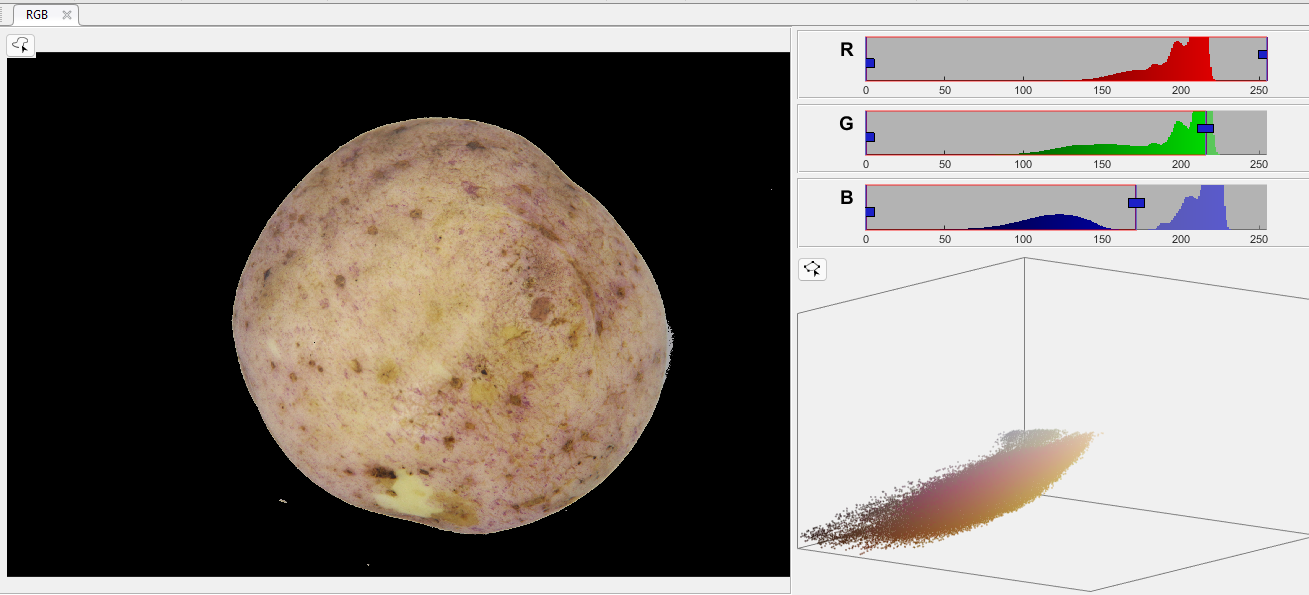
\includegraphics[scale=0.3]{Figs/matlabcv.png}
	\caption{Matlab Color Thresholder}
	\label{fig:matlabcv}
\end{figure}

La herramienta permite, de forma interactiva, crear una función para quitar ciertos colores en el espacio \textit{RGB} de la imagén de muestra, en este caso, se realizó el proceso para retirar el fondo de la imagén de la papa, A este proceso se le conoce como umbralización. \\

Se pretende encontrar el perímetro aproximado de la papa utilizando la función \textit{FindContour} de\textit{OpenCV}, debido a esto, es necesario realizar una serie de transformaciones que conviertan la imágen de muestra, en una imágen binaria (blanco y negro). Se utilizaron los filtros de dilatación y mediana para realizar este proceso como se muestra en la Figura \ref{fig:dilmed}.	

\begin{figure}[ht]
	\centering
	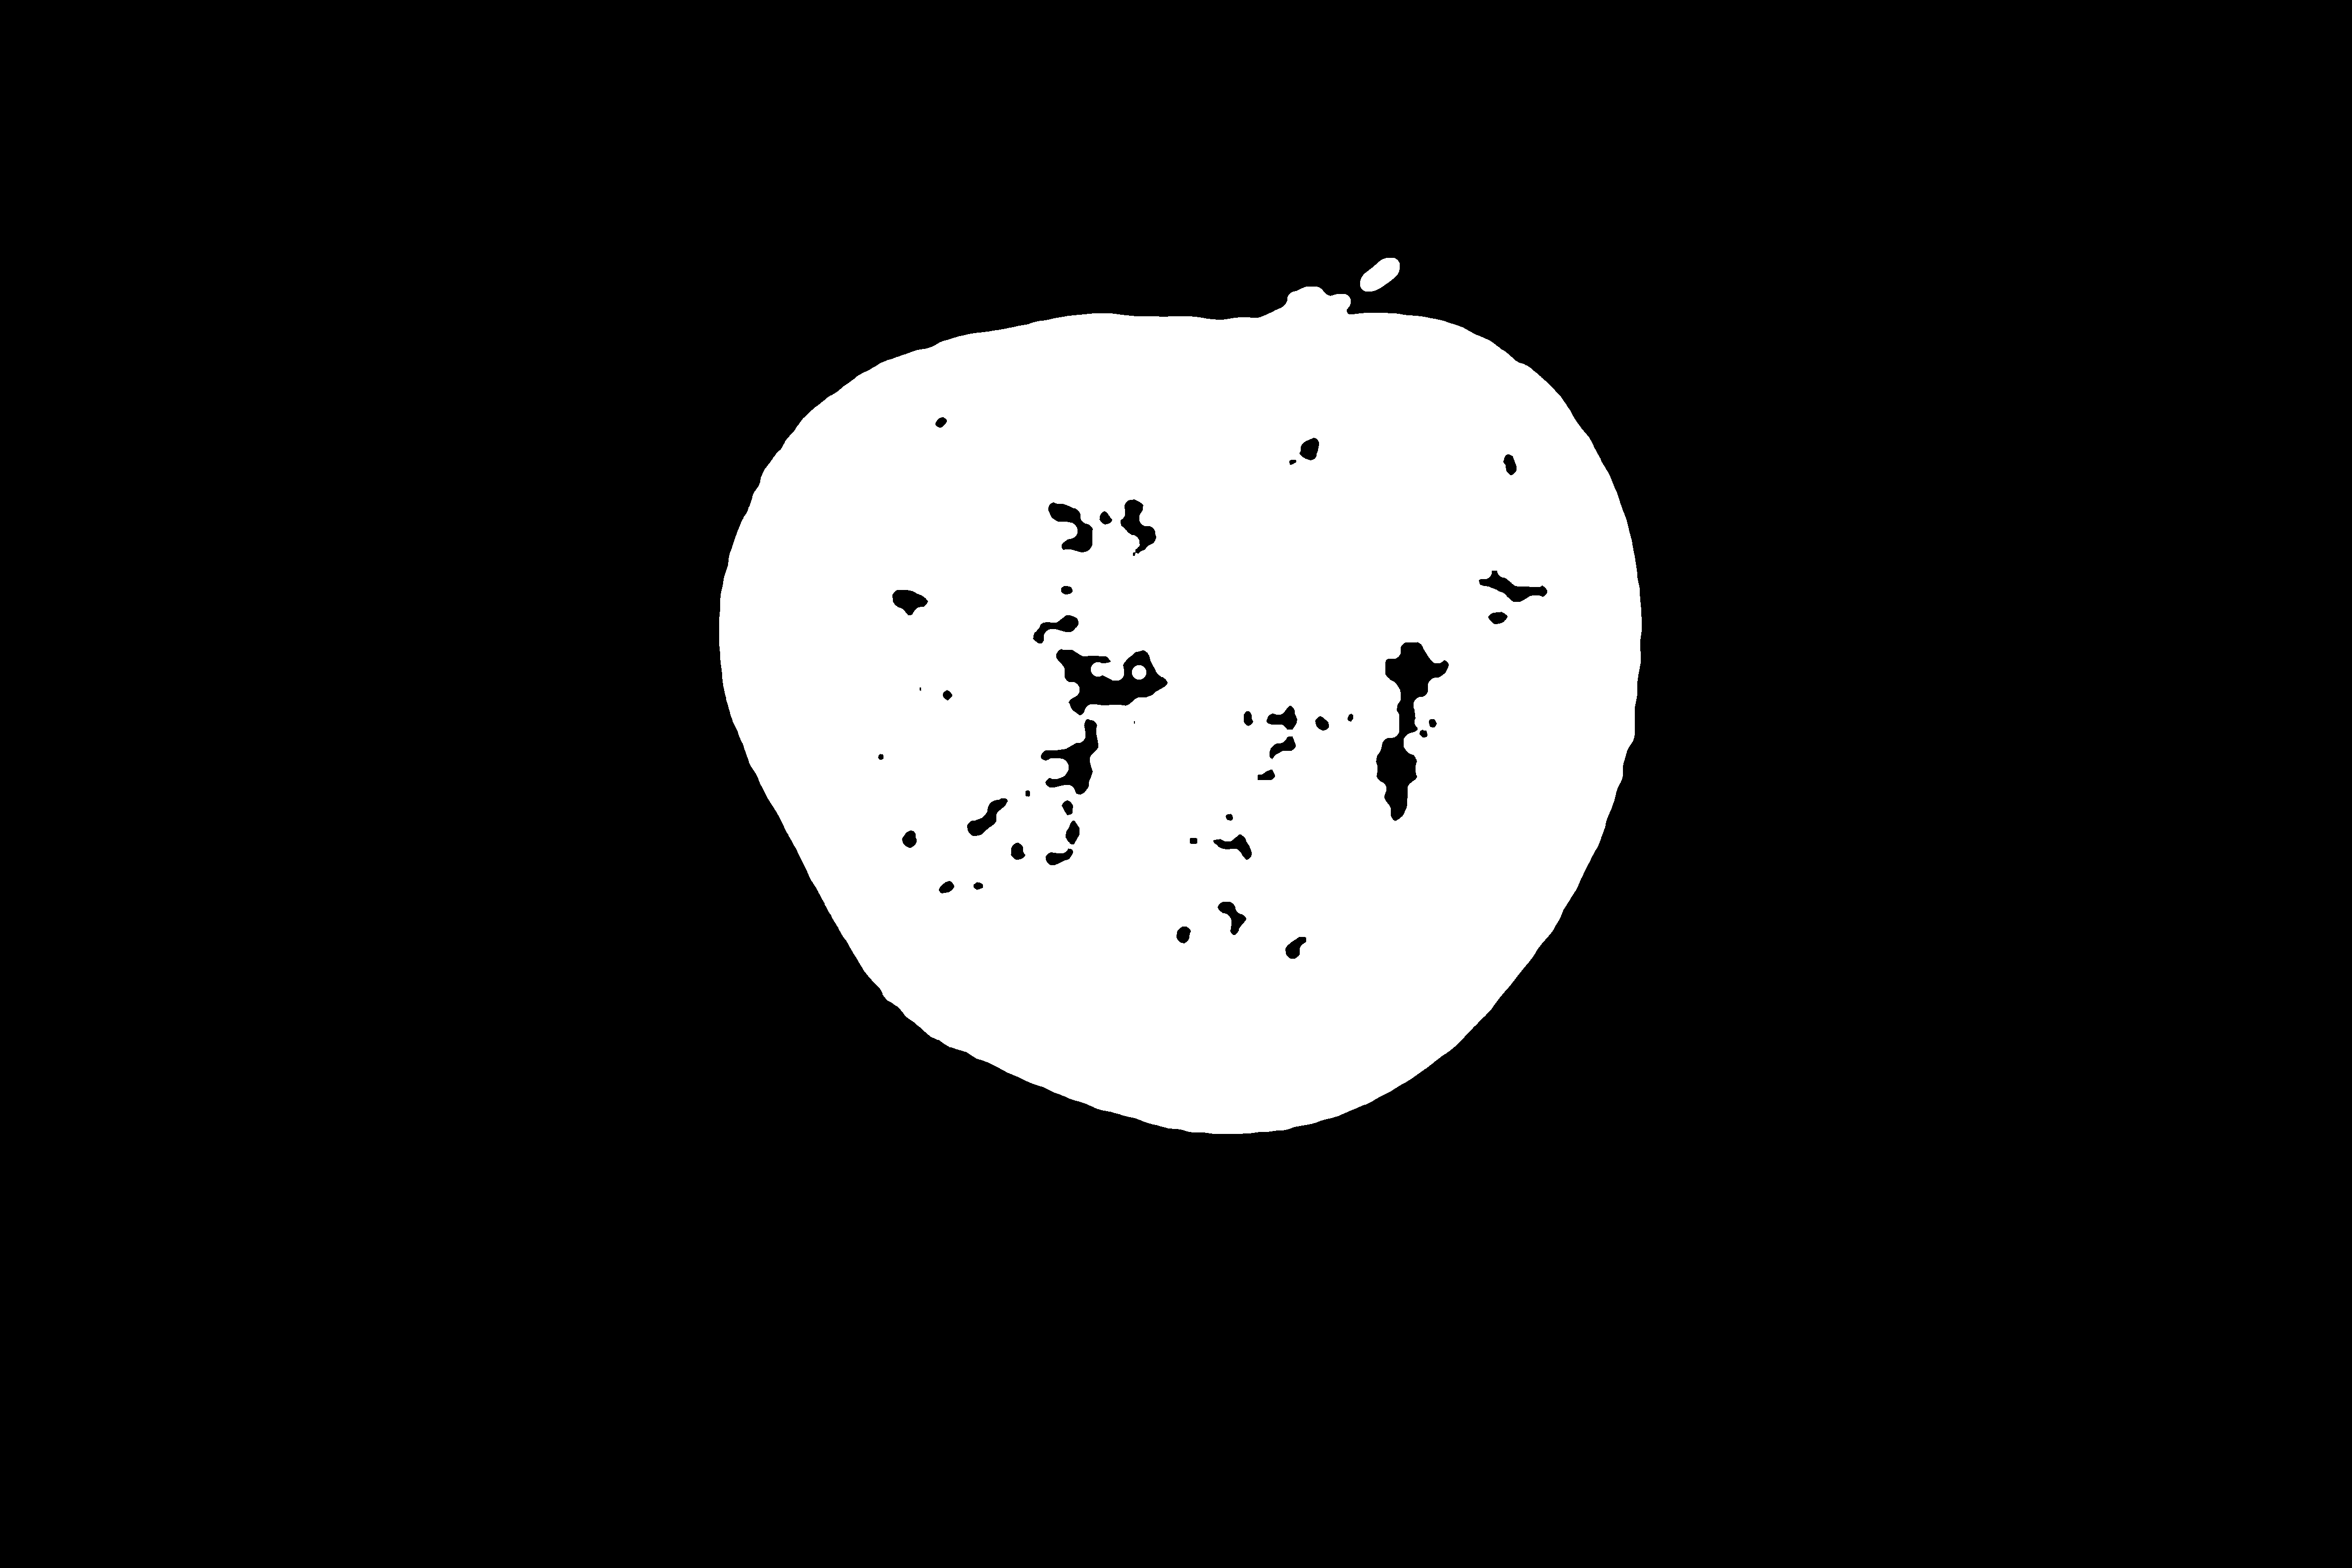
\includegraphics[scale=0.05]{Figs/dilmed.png}
	\caption{Imágen de Muestra Binarizada}
	\label{fig:dilmed}
\end{figure}

Con la imágen aislada de la mayoría de características que puedan interferir en el cálculo del perímetro, utilizando la función de \textit{FindContour}, se puede encontrar y dibujar un perímetro aproximado como se muestra en la Figura \ref{fig:contour}.

\begin{figure}[ht]
	\centering
	\includegraphics[scale=0.05]{Figs/contour.png}
	\caption{Perímetro Aproximado De Las Papas}
	\label{fig:contour}
\end{figure}

En este punto, utilizando la función \textit{ArcLenght} de\textit{OpenCV}, se puede calcular el perímetro del contorno encontrado en cantidad de píxeles. Debido a que las imágenes tomadas para crear el \textit{Dataset} fueron hechas desde una distancia fija desde el lente de la cámara, el tamaño relativo se puede asumuir correcto. Para clasificar estos tamaños, se realizo un estudio en $5$ imágenes de cada tamaño, en donde se calcularon los perímetros, se calculó un promedio y una desviación estádandar, para definir los límites en el tamaño de píxeles por cada tamaño de papa definido. En la Tabla \ref{table:perimetro} se muestran los resultados de estudio realizado.

\newpage	
\begin{table}[ht]
	\centering
	\begin{tabular}{cccccc}
		\hline
		\multicolumn{2}{|c|}{Muy Grande}                                                    & \multicolumn{2}{c|}{Grande}                                                        & \multicolumn{2}{c|}{Mediana}                                                       \\ \hline
		\multicolumn{1}{|c|}{Imagen}            & \multicolumn{1}{|p{2cm}|}{Tamaño del Perimetro} & \multicolumn{1}{c|}{Imagen}            & \multicolumn{1}{|p{2cm}|}{Tamaño del Perimetro} & \multicolumn{1}{c|}{Imagen}            & \multicolumn{1}{|p{2cm}|}{Tamaño del Perimetro} \\ \hline
		\multicolumn{1}{|c|}{0\_0\_0\_1963.jpg} & \multicolumn{1}{c|}{8580,08}              & \multicolumn{1}{c|}{0\_0\_1\_1239.jpg} & \multicolumn{1}{c|}{6524,936741}          & \multicolumn{1}{c|}{0\_0\_2\_2011.jpg} & \multicolumn{1}{c|}{6074,978377}          \\ \hline
		\multicolumn{1}{|c|}{0\_1\_0\_1806.jpg} & \multicolumn{1}{c|}{9523,78}              & \multicolumn{1}{c|}{0\_1\_1\_1828.jpg} & \multicolumn{1}{c|}{6802,549007}          & \multicolumn{1}{c|}{0\_1\_2\_1506.jpg} & \multicolumn{1}{c|}{5.018}                \\ \hline
		\multicolumn{1}{|c|}{1\_0\_0\_0777.jpg} & \multicolumn{1}{c|}{13.275}               & \multicolumn{1}{c|}{1\_0\_1\_0796.jpg} & \multicolumn{1}{c|}{10602,79825}          & \multicolumn{1}{c|}{1\_0\_2\_1995.jpg} & \multicolumn{1}{c|}{5090,177294}          \\ \hline
		\multicolumn{1}{|c|}{1\_1\_0\_0825.jpg} & \multicolumn{1}{c|}{27.830}               & \multicolumn{1}{c|}{1\_1\_1\_0770.jpg} & \multicolumn{1}{c|}{10285,33525}          & \multicolumn{1}{c|}{1\_1\_2\_0857.jpg} & \multicolumn{1}{c|}{5500,756232}          \\ \hline
		\multicolumn{1}{|c|}{0\_0\_0\_1964.jpg} & \multicolumn{1}{c|}{21.607}               & \multicolumn{1}{c|}{0\_0\_1\_1240.jpg} & \multicolumn{1}{c|}{6.726}                & \multicolumn{1}{c|}{0\_0\_2\_2013.jpg} & \multicolumn{1}{c|}{6046,628085}          \\ \hline
		\multicolumn{1}{|c|}{Promedio}          & \multicolumn{1}{c|}{16163,19}             & \multicolumn{1}{c|}{Promedio}          & \multicolumn{1}{c|}{8188,33}              & \multicolumn{1}{c|}{Promedio}          & \multicolumn{1}{c|}{5546,12}              \\ \hline
		\multicolumn{1}{|c|}{Variacion STD}     & \multicolumn{1}{c|}{7425,235484}          & \multicolumn{1}{c|}{Variacion STD}     & \multicolumn{1}{c|}{1846,765787}          & \multicolumn{1}{c|}{Variacion STD}     & \multicolumn{1}{c|}{451,4373313}          \\ \hline
		\multicolumn{1}{|c|}{Limite inferior}   & \multicolumn{1}{c|}{9000,00}              & \multicolumn{1}{c|}{Limite inferior}   & \multicolumn{1}{c|}{6341,56}              & \multicolumn{1}{c|}{Limite inferior}   & \multicolumn{1}{c|}{5094,68}              \\ \hline
		\multicolumn{1}{|c|}{Limite superior}   & \multicolumn{1}{c|}{23588,42}             & \multicolumn{1}{c|}{Limite superior}   & \multicolumn{1}{c|}{9000,00}              & \multicolumn{1}{c|}{Limite superior}   & \multicolumn{1}{c|}{5997,56}              \\ \hline                           
	\end{tabular}
	\caption{Perímetro en Tamaño de Píxeles}
	\label{table:perimetro}
\end{table}

De esta forma, se realiza la clasificación por tamaño en nuevas imágenes de papas, si el valor del perímetro de encuentra dentro de los límites inferior y superior calculados para cada tamaño, la imagen será clasificada de acuerdo a los rangos.


\newpage
\chapter{Prototipo}
En este capitulo se presentan diferentes numerales, para detallar y explicar el prototipo implementado para la clasificación de tubérculos de papa. En el numeral \textit{6.1} se dan a conocer las especificaciones de la maquina implementada. seguido en el numeral \textit{6.2} donde se realiza la descripción de la maquina. En el numeral \textit{6.3} se tiene la descripción del sistema eléctrico y sus componentes, y por ultimo, se termina con los numerales \textit{6.4 y 6.5}, donde se explica la estructura construida para la clasificación de los tubérculos, y se finaliza con el funcionamiento de la maquina.

\section{Especificaciones principales}
Se implementa una banda transportadora, tomada de una maquina selladora de banda continua horizontal FR-900, la cual es impulsada por un motor DC a 220V. Las especificaciones técnicas de la selladora, se presentan en la Tabla \ref{fig:principales}. La máquina se alimenta con $220 \ VAC$ a $50 \ HZ$ y su estructura es en acero inoxidable. 

\begin{table}[ht]
	\centering
	\begin{tabular}{|c|c|c|c|}
		\hline
		\multicolumn{4}{|l|}{\textbf{MOTOR}} \bigstrut\\
		\hline
		\multicolumn{2}{|c|}{REFERENCIA:} & \multicolumn{2}{c|}{ZYT 90-01} \bigstrut\\
		\hline
		\multicolumn{2}{|c|}{CORRIENTE:} & \multicolumn{2}{c|}{0,32 A} \bigstrut\\
		\hline
		\multicolumn{2}{|c|}{VOLTAJE:} & \multicolumn{2}{c|}{220 VDC} \bigstrut\\
		\hline
		\multicolumn{2}{|c|}{VELOCIDAD:} & \multicolumn{2}{c|}{2000 r/min} \bigstrut\\
		\hline
		\multicolumn{2}{|c|}{POTENCIA:} & \multicolumn{2}{c|}{50 W} \bigstrut\\
		\hline
		\multicolumn{4}{|l|}{\textbf{DIMENSIONES}} \bigstrut\\
		\hline
		\multicolumn{2}{|c|}{HORIZONTAL:} & \multicolumn{2}{c|}{850 x 420 x 320 (mm)} \bigstrut\\
		\hline
		\multicolumn{2}{|c|}{VERTICAL:} & \multicolumn{2}{c|}{850 x 320 x 550 (mm)} \bigstrut\\
		\hline
		\multicolumn{2}{|c|}{CONSOLA:} & \multicolumn{2}{c|}{850 x 320 x 1000 (mm)} \bigstrut\\
		\hline
	\end{tabular}%
	\caption{Especificaciones Principales}
	\label{fig:principales}
\end{table}%


\newpage
\section{Descripción de la maquina}
En la Figura \ref{fig:Banda}, se presenta un esquema general de la maquina selladora de banda continua horizontal FR-900, y en la Tabla \ref{table:Banda} se describen las partes presentadas en la Figura \ref{fig:Banda}.
\begin{figure}[ht]
	\centering
	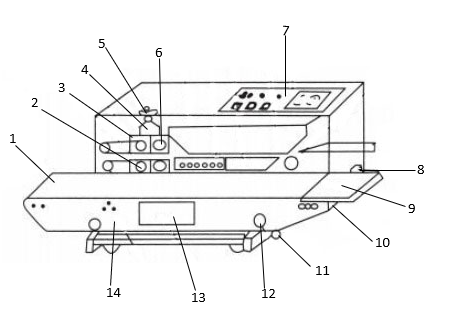
\includegraphics[scale=0.95]{Figs/65.png}
	\caption{Maquina Banda Transportadora}
	\label{fig:Banda}
\end{figure}

\begin{table}[ht]
	\centering
	\begin{tabular}{|p{5cm}|p{8cm}|}
		\hline
		1- Cinta transportadora & 8- Enchufe de corriente y protección \\ 
		\hline
		2- Rueda de goma& 9- Mesa de trabajo fija\\
		\hline
		3- Rodillo de goma& 10- Tornillo de regulación de la elasticidad de las cintas transportadoras\\
		\hline
		4- Asiento rueda de tintorería& 11- Perilla de regulación de la entrada y salida de la estación de transporte\\
		\hline
		5- Rueda reguladora de presión& 12- Perilla de regulación de la altura de la estación transportadora\\
		\hline
		6- Rueda motriz& 13- Placa de identificación\\
		\hline
		7- Caja de Control& 14- Estación de transporte\\
		\hline
	\end{tabular}	
	\caption{Descripción Maquina Transportadora}
	\label{table:Banda}
\end{table}

\newpage
\section{Esquema eléctrico}
En la Figura \ref{fig:Esquema} se presenta las conexiones eléctricas realizadas para el funcionamiento del prototipo, ademas de esto, se anexa en la Tabla \ref{table:esquema} el listado de elementos implementados.  
\begin{figure}[ht]
	\centering
	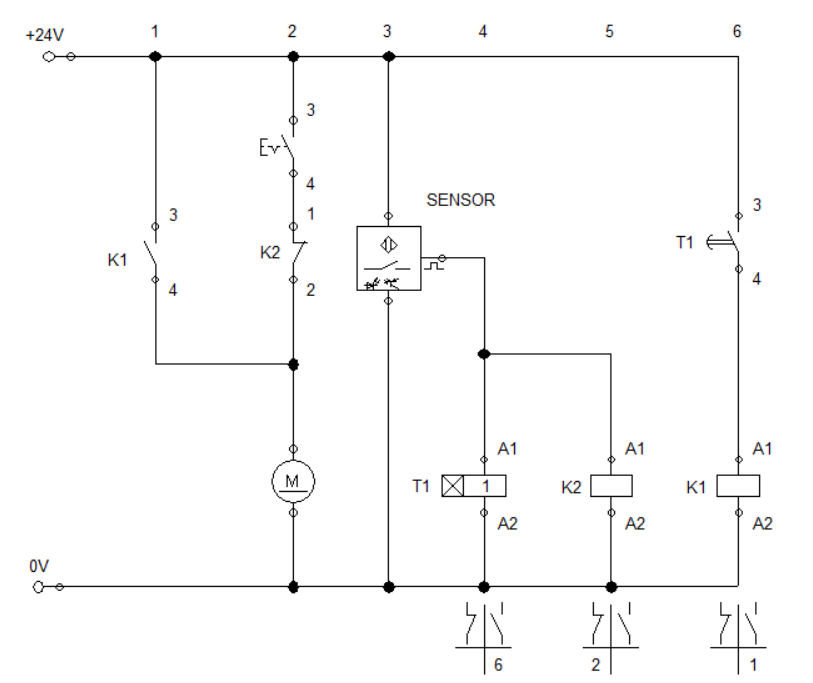
\includegraphics[scale=0.5]{Figs/66.png}
	\caption{Esquema eléctrico}
	\label{fig:Esquema}
\end{figure}

\begin{table}[ht]
	\centering
	\begin{tabular}{|p{2cm}|p{5cm}|p{3cm}|}
		\hline
		SÍMBOLO & NOMBRE & CANTIDAD \\ 
		\hline
		V1 & Fuente de Voltaje & 1 \\
		\hline
		T1 & Temporizador & 1 \\
		\hline
		K1 & Relé & 1 \\
		\hline
		M1 & Motor DC & 1 \\
		\hline
		SENSOR & Sensor Fotoeléctrico & 1 \\
		\hline
		K2 & Relé & 1 \\
		\hline
	\end{tabular}	
	\caption{Elementos Esquema Eléctrico}
	\label{table:esquema}
\end{table}	

\newpage	
\section{Estructura}
La caja elaborada para el análisis de los tubérculos de papas, fue construida en acetato con medidas de, \textit{35 x 25(cm)} las laminas frontal y trasera (Figuras \ref{fig:frontal} y \ref{fig:trasera}), \textit{16 x 25(cm)} lamina superior (Figura \ref{fig:superior}), \textit{20 x 16(cm)} laminas laterales como se muestra en la Figura \ref{fig:lateral}.

\begin{figure}[h!]
	\centering
	\begin{subfigure}{0.45\linewidth}
		\centering
		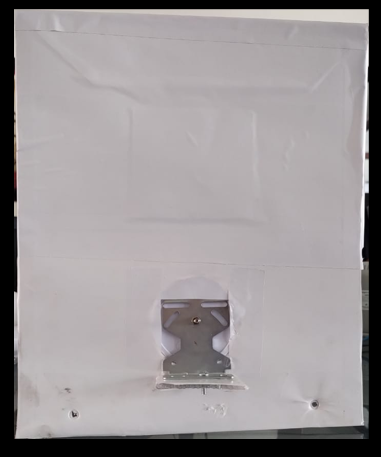
\includegraphics[scale=0.3]{Figs/300.png}
		\caption{Lamina Frontal}
		\label{fig:frontal}
	\end{subfigure}
	\begin{subfigure}{0.45\linewidth}
		\centering
		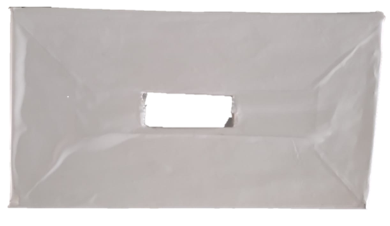
\includegraphics[scale=0.5]{Figs/301.png}
		\caption{Lamina superior}
		\label{fig:superior}
	\end{subfigure}
	\caption{Estructura de Análisis Laminas Principales}
	\label{fig:estructura}
\end{figure} 

\begin{figure}[h!]
	\centering
	\begin{subfigure}{0.45\linewidth}
		\centering
		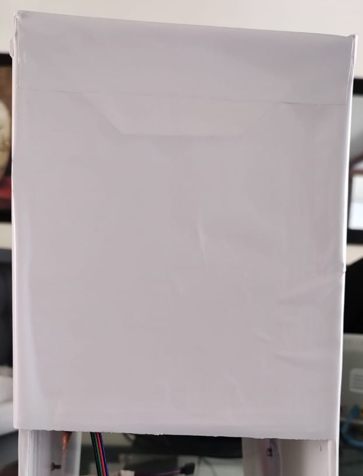
\includegraphics[scale=0.3]{Figs/302.png}
		\caption{Lamina lateral}
		\label{fig:lateral}
	\end{subfigure}
	\begin{subfigure}{0.45\linewidth}
		\centering
		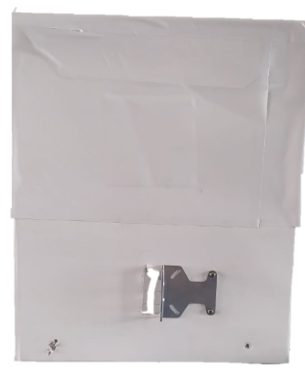
\includegraphics[scale=0.3]{Figs/303.png}
		\caption{Lamina Trasera}
		\label{fig:trasera}
	\end{subfigure}
	\caption{Estructura de Análisis Laminas Laterales}
	\label{fig:estructura}
\end{figure} 


Como se muestra en las Figuras , las laminas fueron diseñadas con las medidas necesarias para posicionar algunos elementos, que permitieran realizar la clasificación de los tuberculos, como lo son bombillos, un sensor optico y una camara web, los cuales seran definidos en los numerales \textit{6.4.1, 6.4.2 y 6.4.3}.

\subsection{Bombillos}
La estructura cuenta con dos agujeros, donde se ubican dos bombillos de luz blanca de 6500 Kelvin de temperatura, para mantener la iluminación fija, a una distancia de 30 cm de todas las fotos, al igual que se tomaron durante la construcción del Dataset.
\subsection{Sensor Fotoeléctrico}
Se implementa un sensor fotoeléctrico, de referencia MAGEWAY, el cual tiene como objetivo detener la banda transportadora una vez el tubérculo de papa se encuentre posicionado bajo la cámara, para realizar su respectiva inspección, el sensor cuenta con las siguientes especificaciones.
\\
\\
\textbf{ESPECIFICACIONES TÉCNICAS:}
\begin{itemize}
	\item Método de detección: retroreflectante.
	\item Ángulo: 1,5 o aprox.
	\item Máx. Rango de detección: 4 m.
	\item Voltaje de alimentación: 12-240 VDC, 24-240V ACBR, Salida: Relé SPDT
	\item Capacidad de salida: 3 A/30 VCC, 3 A/250 VAC.
	\item Temperatura ambiente: -4-131 °F (-20-55 °C).
\end{itemize}

\subsection{Cámara Web}
Para la detección de los tubérculos de papa, se implementa una cámara \textit{Web Camera America Store}, la cual será la encargada de la toma de fotos de los tubérculos, mientras son transportados en la banda transportadora para su análisis.
\\
\\
\textbf{ESPECIFICACIONES TÉCNICAS:}
\begin{itemize}
	\item Lente: Lente de Cristal
	\item Tamaño del artículo: 8 x 4 x 8 cm
	\item Chip DSP: sin controlador
	\item Sensor de imagen: CMOS
	\item Resolución dinámica: 1920 x 1080
	\item Marco: 30 fps
	\item Longitud Focal: 8 mm - infinity
	\item Longitud del Cable: aproximadamente 138 cm
\end{itemize}

\section{Funcionamiento}
Aquí se describe el funcionamiento mecánico de la maquina y el funcionamiento de la red neuronal, la cual fue programada en la tarjeta Jetson Nano para realizar la clasificación de los tubérculos de papa.

\subsection{Funcionamiento Mecánico}
El funcionamiento mecánico inicia conectando la alimentación de la maquina, una vez la maquina se encuentre conectada, el indicador luminoso que se encuentra en el pulsador de inicio, se activará, como se muestra en la Figura \ref{fig:indicador}, esto para dar a conocer que la maquina ya puede entrar en funcionamiento.

\begin{figure}[ht]
	\centering
	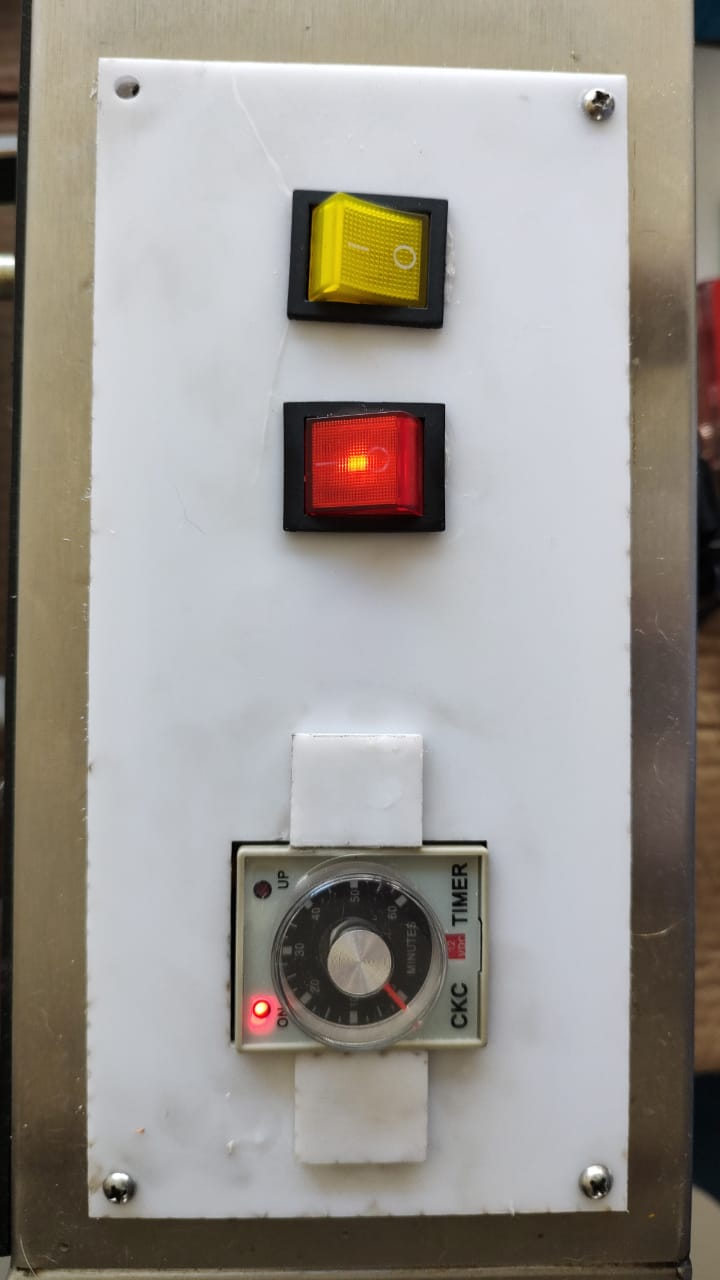
\includegraphics[angle=270, scale=0.21]{Figs/200.jpg}
	\caption{Indicador Luminoso}
	\label{fig:indicador}
\end{figure}

Se presiona el pulsador anteriormente mencionado, y se genera la conmutación del relé para la activación del motor, el cual se encuentra conectado a una caja reductora, que transmite la energía a tres engranajes rectos como se presentan en la Figura \ref{fig:caja}.

\begin{figure}[ht]
	\centering
	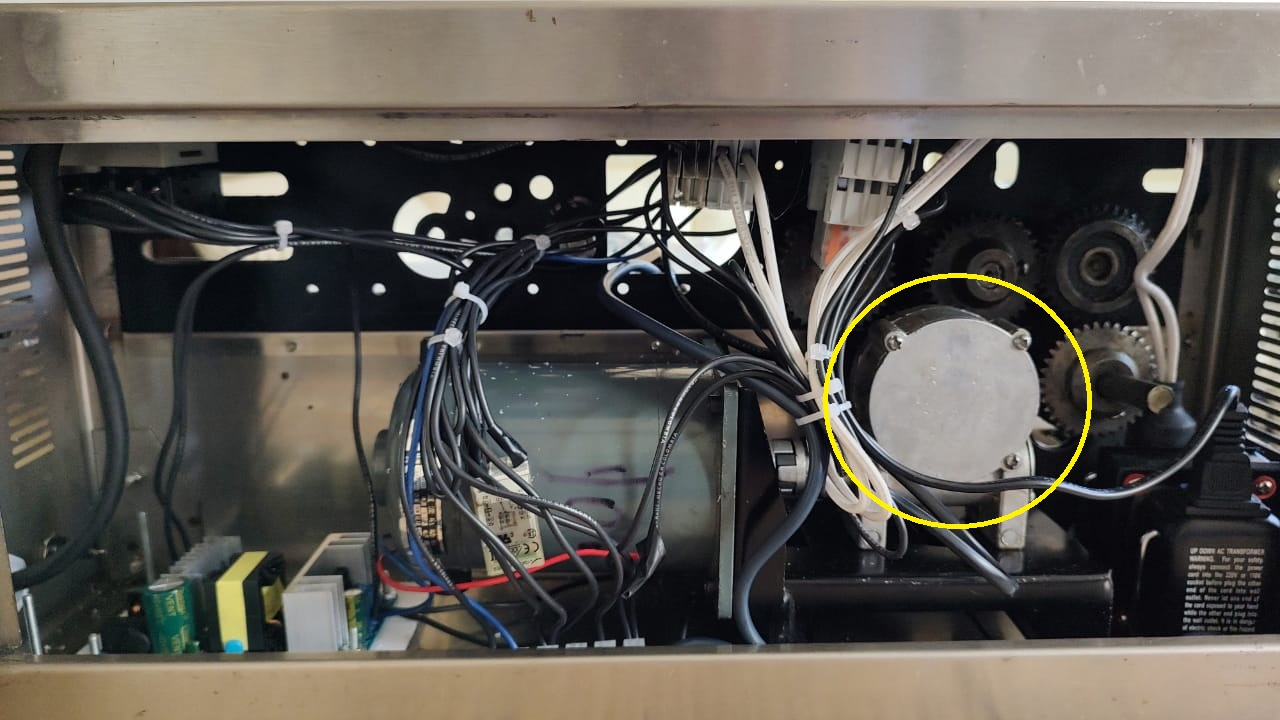
\includegraphics[scale=0.13]{Figs/201.jpg}
	\caption{Caja Reductora De Transmisión A Engranajes Rectos}
	\label{fig:caja}
\end{figure}

En donde el último engranaje se encuentra conectado, y transmite la energía a uno de los rodillos tensores de la banda transportadora, mediante un eje, como se aprecia en la Figura \ref{fig:eje}, con el fin de generar el movimiento de la banda. 

\newpage
\begin{figure}[ht]
	\centering
	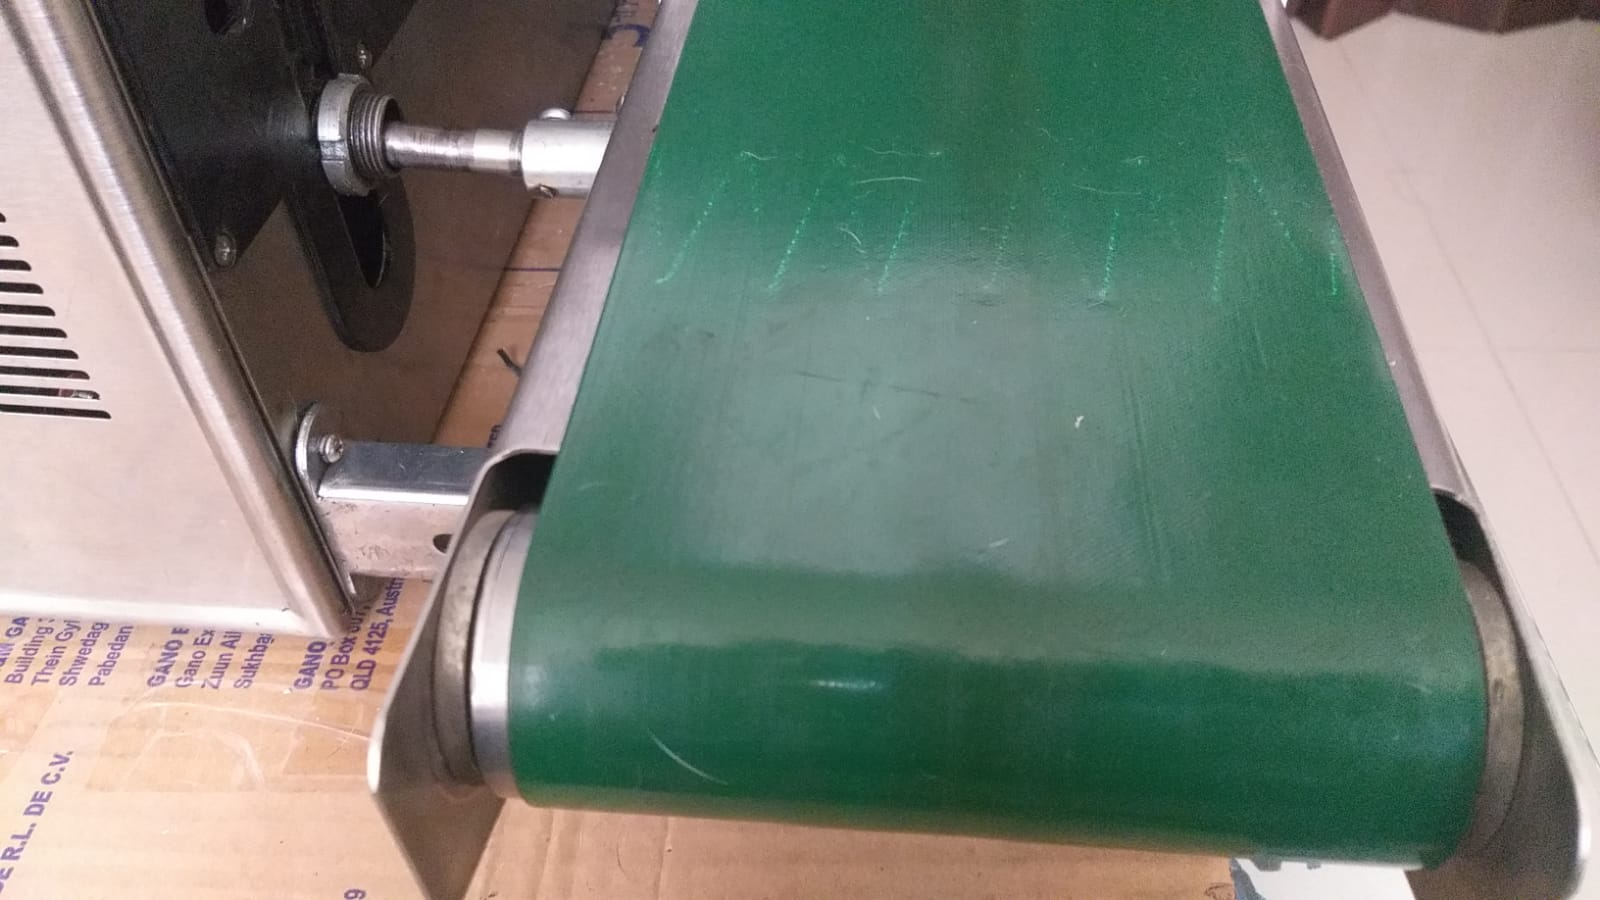
\includegraphics[angle=270, scale=0.21]{Figs/202.jpg}
	\caption{Conexión Engranajes y Rodillo Tensor}
	\label{fig:eje}
\end{figure}


Una vez se inicia el movimiento de la banda transportadora, este seguirá hasta que el tubérculo entre en contacto con el con la luz infrarroja del sensor foto eléctrico, como se observa en la Figura \ref{fig:sensor}, cuando el sensor detecte el tubérculo, la señal enviada detendrá la banda y activara un timer de un segundo, esto con el fin de permitir que la cámara tome la foto del tubérculo, y la envié a la red neuronal para su análisis el cual se explicará en la sección \textit{6.5.2 Implementación en Sistema Embedido}. Culminado el tiempo establecido en el timer, la banda continuara su movimiento para desplazar y continuar con la clasificación de los tubérculos.

\begin{figure}[ht]
	\centering
	\includegraphics[scale=0.15]{Figs/203.jpg}
	\caption{Detección del sensor fotoeléctrico}
	\label{fig:sensor}
\end{figure}


\subsection{Implementación en Sistema Embebido}

Para el funcionamiento del algoritmo en tiempo real, en el prototipo construido, se utilizó una tarjeta de desarrollo Nvidia Jetson Nano $2 \ GB$, debido a que cuenta con una tarjeta gráfica y está diseñada para ejecutar modelos de redes neuronales. La implementación del algoritmo, debido a que la red fue entrenada con imágenes de tubérculos de papa estáticas, se realizó de igual forma.\\

El algoritmo captura una foto desde la webcam, realiza el procesamiento en la red neuronal y posteriormente, la clasificación por tamaño. Los resultados de cada imágen son mostrados por consola y la imágen capturada es guardada en formato $.jpg$, con la información de las predicciones, para verificar si la clasificación fue correcta. La imagen \ref{fig:implementacion}, muestra una de las papas pasando dentro de las estructura hecha para la clasificación.

\begin{figure}[ht]
	\centering
	\includegraphics[scale=0.25]{Figs/implementacion.jpg}
	\caption{Tubérculo de Papa Dentro de La Estructura}
	\label{fig:implementacion}
\end{figure}

Se realizó un experimento con 50 papas de las diferentes clases, para verificar la precisión del algoritmo. La Tabla \ref{table:res} muestra los resultados de algunas de las papas utilizadas.

\begin{table}[ht]
	\centering
	\begin{tabular}{|cc|cc|}
		\hline
		\multicolumn{2}{|c|}{Real}                 & \multicolumn{2}{c|}{Prediccion}           \\ \hline
		\multicolumn{1}{|c|}{Clase}   & Tamaño     & \multicolumn{1}{c|}{Clase}   & Tamaño     \\ \hline
		\multicolumn{1}{|c|}{Clase 1} & Grande     & \multicolumn{1}{c|}{Clase 1} & Mediano    \\ \hline
		\multicolumn{1}{|c|}{Clase 1} & Muy Grande & \multicolumn{1}{c|}{Clase4}  & Muy Grande \\ \hline
		\multicolumn{1}{|c|}{Clase 4} & Mediana    & \multicolumn{1}{c|}{Clase 4} & Mediana    \\ \hline
		\multicolumn{1}{|c|}{Clase 3} & Grande     & \multicolumn{1}{c|}{Clase 3} & Grande     \\ \hline
		\multicolumn{1}{|c|}{Clase 2} & Mediana    & \multicolumn{1}{c|}{Clase 2} & Mediana    \\ \hline
		\multicolumn{1}{|c|}{Clase 1} & Mediana    & \multicolumn{1}{c|}{Clase 2} & Grande     \\ \hline
		\multicolumn{1}{|c|}{Clase 4} & Grande     & \multicolumn{1}{c|}{Clase 3} & Grande     \\ \hline
		\multicolumn{1}{|c|}{Clase 3} & Mediana    & \multicolumn{1}{c|}{Clase 3} & Mediana    \\ \hline
		\multicolumn{1}{|c|}{Clase 1} & Mediana    & \multicolumn{1}{c|}{Clase 1} & Mediana    \\ \hline
	\end{tabular}
	\caption{Resultados Papas Predichas}
	\label{table:res}
\end{table}


De las 50 papas utilizadas para la verificación, se obtuvo un resultado de $80\%$ de clases con correcta predicción y $88\%$ de tamaños correctamente clasificados. Esto da una precisión total de $85\%$ para las papas que fueron correctamente clasificadas en ambas categorías.\\

El tiempo de ejecución del algoritmo, desde el momento en el que toma la foto y la procesa, hasta que realiza la clasificación, varia entre los $2$ y $3$ segundos. El tiempo que demora la papa en llegar desde el comienzo de la banda transportadora, hasta la posición dentro de la estructura de análisis, es de $7$ segundos, por lo tanto, se puede asumir un tiempo promedio de $10$ segundos en analizar 1 tubérculo de papa. Este prototipo clasificaría $100$ tubérculos de papa cada $15$ minutos.	 	

\chapter{Trabajo Futuro}

Debido a que el desarrollo del proyecto es un prototipo, la máquina puede ser mejorada para realizar la clasificación mecánica de las diferentes categorías, de igual forma, se puede implementar un variador para que la banda sea más rápida que el movimiento actual, mejorando así la velocidad de clasificación.\\

La red neuronal artificial que se obtuvo con una precisión superior al $83\%$, puede ser mejorada de tal manera que se puedan obtener precisiones superiores al $90\%$, para mejorar los resultados de las predicciones finales. Esto se puede lograr enriqueciendo el \textit{Dataset}, mejorando la distribución de los datos iniciales, de manera que sean proporcionales entre sí y realizando una optimización de hiperparámetros, teniendo en cuenta diferentes parámetros utilizados en este proyecto. Si se desea realizar una mejor optimización, el poder de computo necesario para realizarla debe ser muy superior, en las condiciones actuales, la optimización tomó un tiempo de $6$ horas por cada modelo en el que se aplicó.\\

Los tiempos de ejecución del algoritmo implementado en el sistema embebido, se deben mejorar, para que el prototipo sea viable en la agricultura de precisión. Mejor capacidad de procesamiento en la tarjeta de desarrollo escogida y mejorar la sintaxis y consumo de memoria por parte del diseño del algoritmo hecho en \textit{Python}.










